\documentclass[a4paper,12pt,english,final]{epsc_tfc_pfc}
%% a4paper: mida paper. No tocar
%% 12pt: mida de la font. No tocar

%%  - OPCIONS A CONFIGURAR:
%%     - Estat del document: final o draft
%%       NOTA: Draft no inserta les figures i indica quan el text sobrepassa els marges.

%%  - IDIOMES QUE S'USARAN EN EL DOCUMENT: catalan, spanish, english, french...
%%    NOTA: per canviar d'idioma al mig del document usar:
%%          \selectlanguage{nom_idioma}
\usepackage[english,catalan]{babel}

%%%%%%%%%%%%%%%%%%%%%%%%%%%%%%%%%%%%%%%%%%%%%%%%%%%%%%%%%%%%%%%%%%%%%%%%%%%%%


%%% PAQUETS LATEX RECOMANABLES A UTILITZAR
%%%%%%%%%%%%%%%%%%%%%%%%%%%%%%%%%%%%%%%%%%%%%%%%%%%%%%%%%%%%%%%%%%%%%%%%%%%%%
%%% NOTA: es possible que algunes distribuicions Linux o Windows 
%%%       no portin aquests paquets instal�lats per defecte.

%% El paquet isolatin1 �s extramadament �til. 
%% Permet escriure els accents directament amb l'editor de texte
%% sense haver de fer coses com per exemple: introducci\'o
\usepackage[latin1]{inputenc}             

%% S�mbols matem�tics de la American Mathematical Society
\usepackage{amssymb,amsmath,amsfonts}

\usepackage{titlesec}

%% Glossaries
%\usepackage[nonumberlist,section=chapter]{glossaries}
\usepackage{glossaries}
\makeglossaries

%% El paquet array proporciona eines molt �tils a l'hora de fer 
%% equacions amb matrius
\usepackage{array}             

%% Permet fer taules fusionant cel�les de files consecutives
%\usepackage{multirow}          

%% Permet canviar els colors del document
%\usepackage{color,colortbl}
\usepackage{float}

\restylefloat{table}

\usepackage{textcomp}

\usepackage[export]{adjustbox}

\usepackage{times}

%\url
\usepackage{url}

\begin{document}
\pagestyle{empty}
%%%%%%%%%%%%%%%%%%%%%%%%%%%%%%%%%%%%%%%%%%%%%%%%%%%%%%%%%%%%%%%%%%%%%%%%%%%%%
%%%%%%%%%%%%%%%%%%%%%%%%%%%%%%%%%%%%%%%%%%%%%%%%%%%%%%%%%%%%%%%%%%%%%%%%%%%%%

%% IDIOMA PRINCIPAL DEL DOCUMENT
%%%%%%%%%%%%%%%%%%%%%%%%%%%%%%%%%%%%%%%%%%%%%%%%%%%%%%%%%%%%%%%%%%%%%%%%%%%%%
\selectlanguage{english}

%%%%%%%%%%%%%%%%%%%%%%%%%%%%%%%%%%%%%%%%%%%%%%%%%%%%%%%%%%%%%%%%%%%%%%%%%%%%%
%% PORTADA
%%%%%%%%%%%%%%%%%%%%%%%%%%%%%%%%%%%%%%%%%%%%%%%%%%%%%%%%%%%%%%%%%%%%%%%%%%%%%
%% Portada generada autom�ticament a partir del fitxer de dades
\portada

%% RESUM
%%%%%%%%%%%%%%%%%%%%%%%%%%%%%%%%%%%%%%%%%%%%%%%%%%%%%%%%%%%%%%%%%%%%%%%%%%%%%
% NOTA: la longitud passada com a parametre d'entrada 
%       s'ha d'ajustar ``a ull'' fins que el requadre del resum ocupi tota la pagina 
\begin{resum}{10cm}
Aquest document cont� les pautes del format de presentaci� del treball o projecte de final de carrera. En tot cas, cal tenir en compte el que estableix la ``Normativa del treball de fi de carrera (TFC) i del projecte de fi de carrera (PFC)'' aprovada per la Comissi� Permanent de l'EPSC, especialment l'apartat ``Requeriments del treball''.
\end{resum}

%% OVERVIEW
%%%%%%%%%%%%%%%%%%%%%%%%%%%%%%%%%%%%%%%%%%%%%%%%%%%%%%%%%%%%%%%%%%%%%%%%%%%%%
% NOTA: la longitud passada com a parametre d'entrada 
%       s'ha d'ajustar ``a ull'' fins que el requadre del resum ocupi tota la pagina 
\begin{overview}{11cm}
This document contains guidelines for writing your TFC/PFC. However, you should also take into consideration the standards established in the document Normativa del treball de fi de carrera (TFC) i del projecte de fi de carrera (PFC), paying special attention to the section Requeriments del treball, as this document has been approved by the EPSC Standing Committee
\end{overview}

%% DEDICATORIA (opcional)
%%%%%%%%%%%%%%%%%%%%%%%%%%%%%%%%%%%%%%%%%%%%%%%%%%%%%%%%%%%%%%%%%%%%%%%%%%%%%
\begin{dedicatoria}
Escriure aqu� opcionalment la dedicat�ria.
\end{dedicatoria}

%% INDEX de continguts
%%%%%%%%%%%%%%%%%%%%%%%%%%%%%%%%%%%%%%%%%%%%%%%%%%%%%%%%%%%%%%%%%%%%%%%%%%%%%
\thispagestyle{empty} 
\tableofcontents
\cleardoublepage

%% INDEX de figures (opcional, comentar les 3 linies si no es desitja)
%%%%%%%%%%%%%%%%%%%%%%%%%%%%%%%%%%%%%%%%%%%%%%%%%%%%%%%%%%%%%%%%%%%%%%%%%%%%%
\thispagestyle{empty}
\listoffigures
\cleardoublepage

%% INDEX de taules (opcional, comentar les 3 linies si no es desitja)
%%%%%%%%%%%%%%%%%%%%%%%%%%%%%%%%%%%%%%%%%%%%%%%%%%%%%%%%%%%%%%%%%%%%%%%%%%%%%
\thispagestyle{empty}
\listoftables
\cleardoublepage

%%%%%%%%%%%%%%%%%%%%%%%%%%%%%%%%%%%%%%%%%%%%%%%%%%%%%%%%%%%%%%%%%%%%%%%%%%
%%%%%%                    INTRODUCCI�                          %%%%%%%%%%%
%%%%%%%%%%%%%%%%%%%%%%%%%%%%%%%%%%%%%%%%%%%%%%%%%%%%%%%%%%%%%%%%%%%%%%%%%%
%% NOTA: El text passat com a parametre d'entrada 
%%       �s ''introducci�'' amb l'idioma en que es redacti el projecte
\pagestyle{fancy} 

\begin{intro}{Introduction} 
The aim of this thesis is port an existing operating system called Micro Framework developed by Microsoft. Micro Framework is the smallest version of .NET for very resource-constrained devices. This port should let applications using this framework run on any Linux device capable of use Input/Output ports and SPI, UART communication standards.
There is no official implementation of this framework for complete operating systems, in example, Windows or Linux.

The reason of this port is try to migrate a Wireless Sensor Network (WSN) Gateway that currently uses MicroFramework and Netduino Plus which is a constrained-device. But this gateway it's getting out of system resources, so in order to keep the existing code a solution has been proposed, make able to run this software on a Linux device.

In this case, the deployment device will be a RaspberryPi which is a low end computer similar to a Pentium II in terms of computing power. This computer offers a set of interesting things in terms of this thesis, basically it has exposed Input/Output ports as a GPIO. Over this GPIOs it's possible to use SPI, I$^{2}$C and UART communication buses.

After achieving this, there is a second goal which consists of help and test the development of a code translating tool called AlterNative which is being developed by Alex Albal� and Juan L�pez. This translator is capable to get a source code from a C\# binary and translate it to C++ trying to get better performance than C\#. On the other hand, taking the benefit of the C++, the translated code should be able to execute between different operating systems (Windows, Linux and MacOSX and also mobile devices as Android).

\end{intro}

\pagestyle{fancy} 

%%%%%%%%%%%%%%%%%%%%%%%%%%%%%%%%%%%%%%%%%%%%%%%%%%%%%%%%%%%%%%%%%%%%%%%%%%
%%%%%% INCLOURE A PARTIR D'AQU� TOTS ELS CAP�TOLS DE LA MEMORIA   %%%%%%%%
%%%%%%%%%%%%%%%%%%%%%%%%%%%%%%%%%%%%%%%%%%%%%%%%%%%%%%%%%%%%%%%%%%%%%%%%%%

%% First include Glossary to be used in the following chapters
%% INDEX de glossari
%%%%%%%%%%%%%%%%%%%%%%%%%%%%%%%%%%%%%%%%%%%%%%%%%%%%%%%%%%%%%%%%%%%%%%%%%%%%%\\
\thispagestyle{empty}
\newglossaryentry{SPI}{name={SPI},description={Serial Peripheral Interface}}
\newglossaryentry{IRQ}{name={IRQ},description={Interrupt Request}}
\newglossaryentry{BCM2835}{name={BCM2835},description={ARMv6 CPU mounted on the RaspberryPi}}


%\printglossaries
%\cleardoublepage

%% Include the chapters
\chapter{Project overview}\label{C:project-overview}
This project was proposed by AlterAid, a company which is working on several ways to help in taking care of the health of our elderly, or in general, anyone that is relevant to our lives.

This company is working on two different projects that combine together. The first one is called aaaida, which consists of a social network where people can stay alert about its relatives, upload information about its health or watch recommendations from doctors or other professionals. On the other side, and on a more hardware oriented development, they are creating a Wireless Sensor Network called HomeSense that once deployed in a house will be able to collect relevant information from those sensors in the home and allow other people to know if the daily life of the resident's house is going normal, or something is happening.

\section{HomeSense}\label{S:HomeSense}
HomeSense is a Wireless Healthcare Sensor Platform created with the aim of control and care taking of the elderly and relatives. Actually it uses a Netduino Mini board which makes the function of the gateway which controls the sensor network, receiving all the data and uploading to aaaida platform through Internet.
\\
In the house, the communication is carried on using little sensors capable of fetching data in different situations (for example the opening of a drawer or a medicine cabinet). It is also possible to install the sensors on doors in order to know if they are opened or closed, or in any place where is interesting to acquire information from the environment, house or residents. These sensors make use of nRF24LE1 \gls{SoC} with a low-power RF \gls{ISM} band on 2.4GHz from Nordic Semiconductor.
\\
The communication protocol designed for HomeSense is similar to a star network with multi-hop transmissions so it becomes a tree-star topology. The nodes mainly send information to the gateway because this is on charge of upload the information to the Internet, but they are also able to communicate with other nodes.
\\
The gateway system has been entirely developed using .NET Micro Framework and deployed on a Netduino Mini. The mesh protocol has been defined internally on the company while it uses third-party hardware to create the physical links of the network.

\begin{figure}[H]\begin{center}
 \centering
  \captionsetup{justification=centering}
  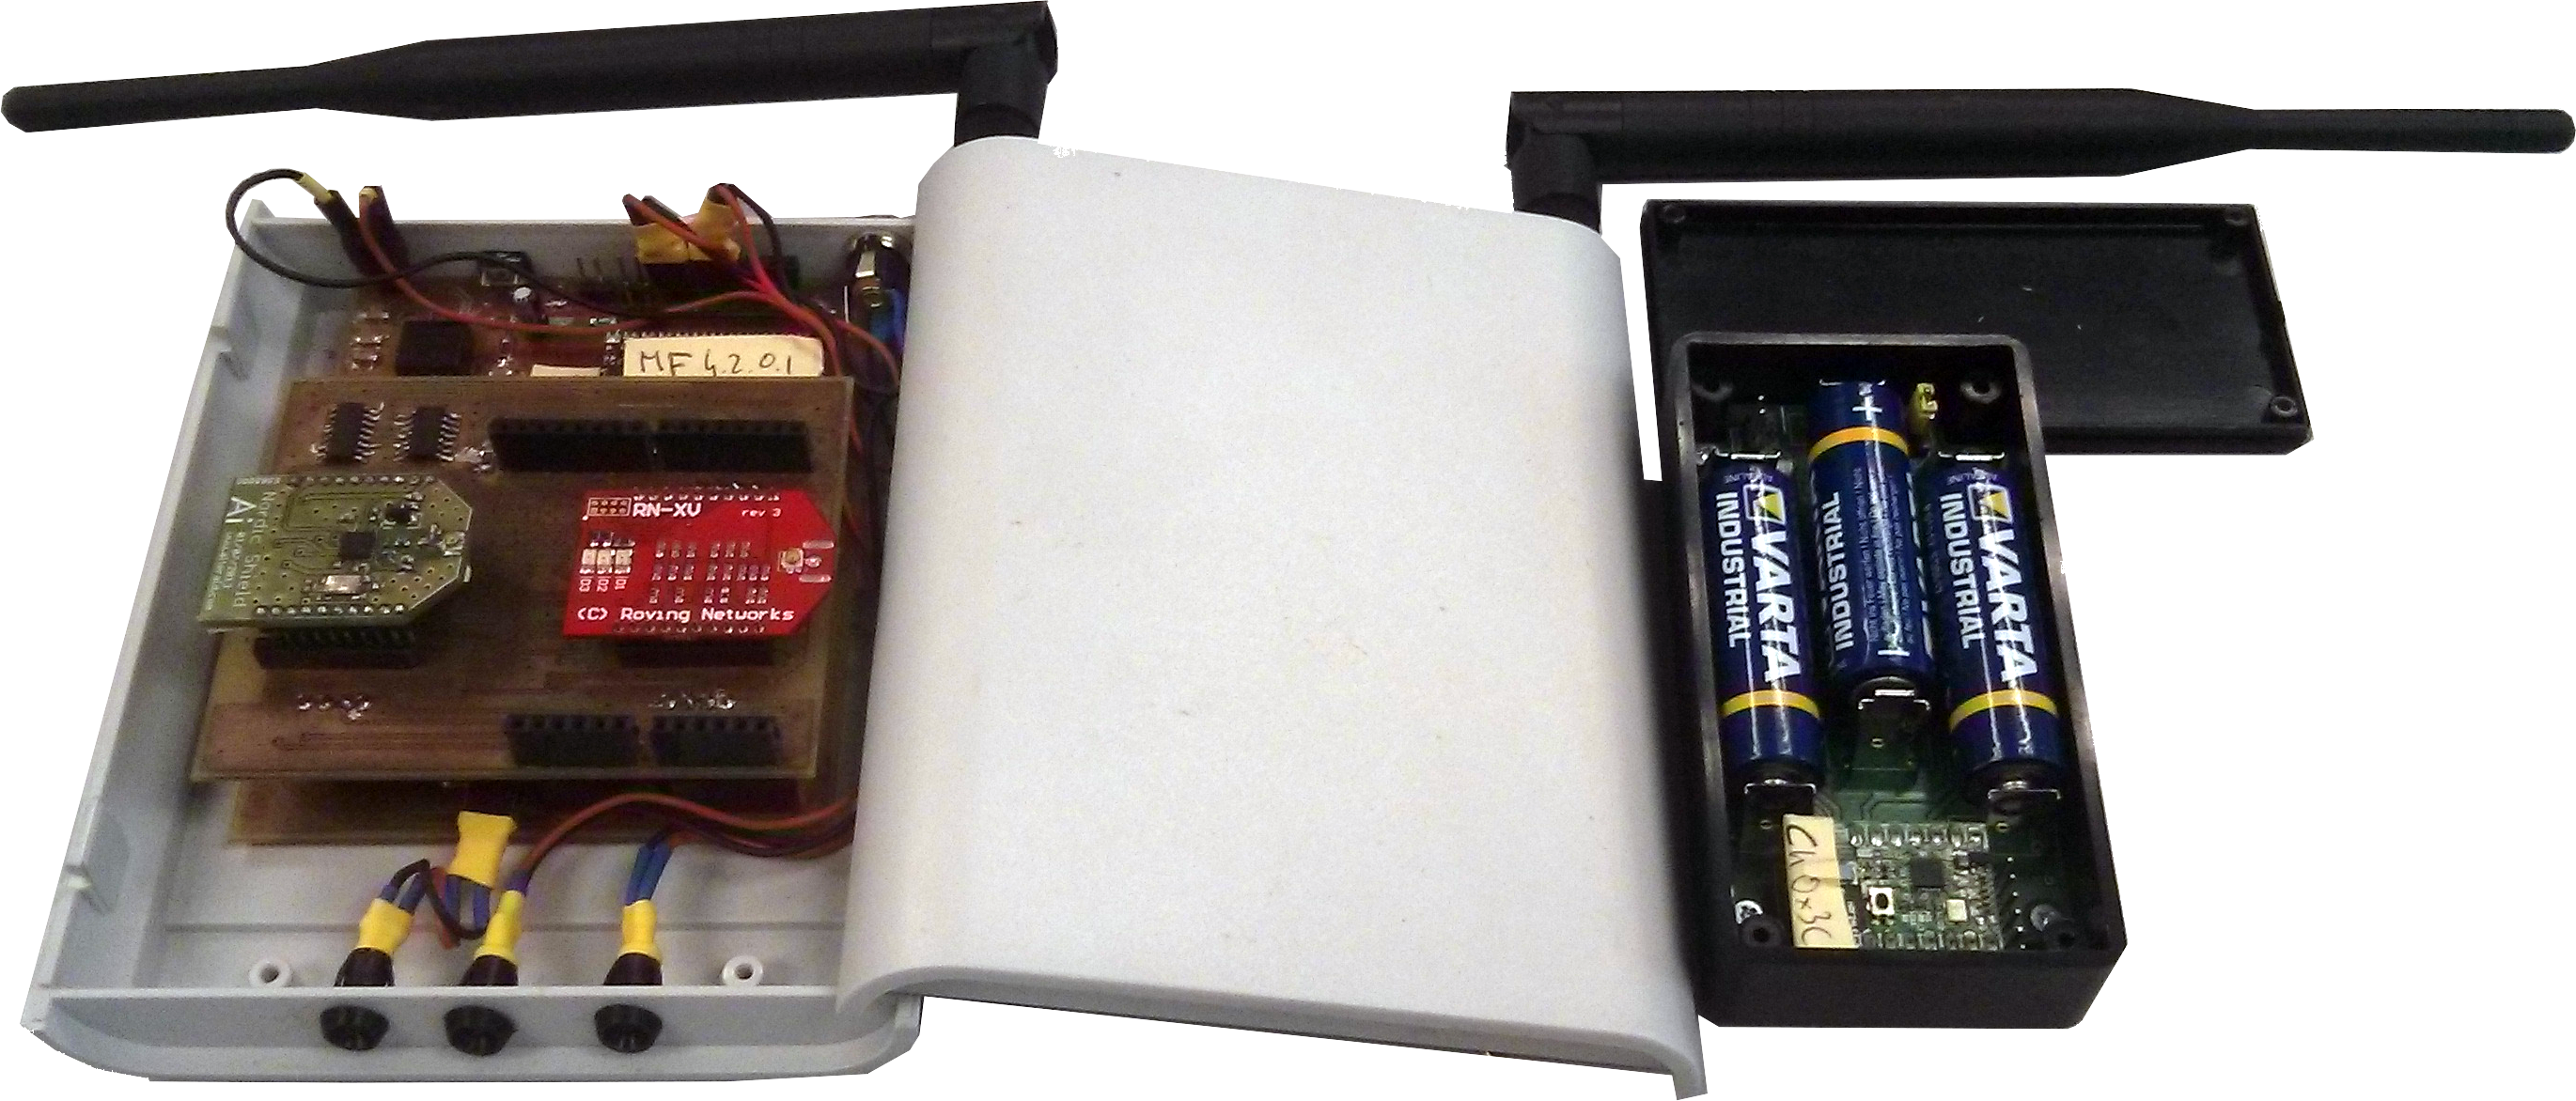
\includegraphics[width=0.7\textwidth]{pictures/proposal/homesense}
  \caption{Sensor on the left and HomeSense gateway on the right \label{fig:Proposal-HomeSense}}
\end{center}\end{figure}

\section{AlterNative}\label{S:Proposal-AlterNative}
AlterNative is a language translating tool created by Alex Albal\'{a} and Juan L\'{o}pez. It can translate a compiled (.NET) assembly or library to standard C++ code. Basically this program decompiles the file to be translated, then it sketches how the program works, which are its classes, functions, nodes, etc and then start translating step-by-step all the program. After that, it links the necessary C++ libraries to work, ones are from boost library, and the other ones are self-written to behave like the original C\# classes.
\\
It is interesting to emphasize that the main difference of this translator between the other existing ones is that it tries to generate a code practically identical to the original C\# source code. By doing this, the resulting C++ source is really easy to read for people not used to C++ syntax and language.
\begin{figure}[H]\begin{center}
 \centering
  \captionsetup{justification=centering}
 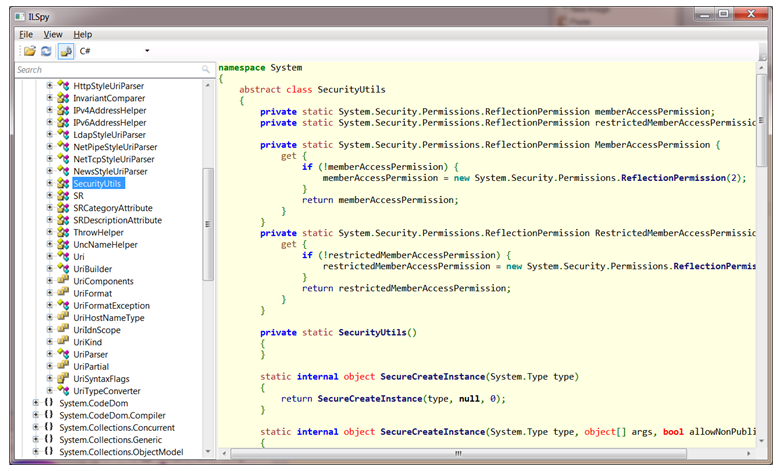
\includegraphics[scale=0.65]{pictures/proposal/alternativeUI}
  \caption{AlterNative interface \label{fig:Proposal-AN}}
\end{center}\end{figure}

\section{Thesis Proposal}\label{S:Proposal-Thesis-Proposal}
After introducing HomeSense and AlterNative is time to explain the thesis proposal itself because it is related to the applications mentioned above. The proposed project is to take the code of the HomeSense gateway, which is written using Micro Framework, and make it run in a Linux device instead of a Netduino Mini because it is getting limited in terms of capabilities, performance and expansion for future characteristics.
\\
The idea is to take the gateway code and port it to other devices capable of use minimum GPIO, interrupts from this ports, the SPI communication protocol and UART because all of them are used in the HomeSense source code. It is important to point that the implemented classes must be similar to the Micro Framework code to avoid major changes on the HomeSense program. Minor changes such as port renaming and communication module name changing are acceptable because they do not alter the original execution flow and design architecture. But not only this should be done on HomeSense, it is interesting to make portable between different hardware platforms any code that runs over Micro Framework.
\\
After accomplishing with this first goal, the second part of the thesis is to use AlterNative to translate the IOSharp library to C++ in order to increase and analyse the performance of IOSharp running on C++ instead of C\#. To accomplish with this objective, some C++ libraries must be written in order to translate IOSharp.

\subsection{Objectives}\label{SS:Proposal-Objectives}
The proposed objectives are listed below explaining briefly each one:  
\begin{itemize}
	\item \textbf{IOSharp:} objectives to be accomplished during the first part of this thesis.
		\begin{itemize}
		\item \textbf{GPIO:} Simple I/O functions (Input, Output ports).
		\item \textbf{Interrupts:} enable interrupts through GPIOs.
		\item \textbf{SPI:} get a working SPI bus on the implementation.
		\item \textbf{UART:} get a functional SerialPort
		\item \textbf{HomeSense:} deploy this WSN as a functional test to show the correct function of the library.
		\end{itemize}
	\item \textbf{AlterNative:} second part of the thesis involving the code translation tool.
		\begin{itemize}
		\item \textbf{Cross-Platform:} although one of the goals of AlterNative is produce a cross-platform source code, it only runs on Windows so Linux or MacOSX use are unable to use this tool because of the graphic dependencies. In this case, the code must be analysed and modified to produce a cross-platform program.
		\item \textbf{Library:} write the necessary methods to let IOSharp be translated.
		\item \textbf{Tests:} write functional tests to determine the correct functionality of the library.
		\item \textbf{Performance analysis:} do some performance analysis to check the performance increase when the code is translated.
		\item \textbf{Translate HomeSense:} do a complete translation of the WSN platform using AlterNative.
		\end{itemize}
\end{itemize}


\section{Document Structure}\label{SS:Proposal-Doc-Structure}
This document is structured on seven chapters that shows the project definition when this thesis was proposed, then a state of the art shows the current technologies or systems that are similar to this thesis. Then the development steps are enumerated where GPIO, interrupts, SPI and UART are involved. Another chapter is dedicated to the functional tests to proof that the IOSharp proposed objectives where done. After these tests an introduction to AlterNative is done along with the performance tests chapter which shows the results for the AlterNative part. Finally, the conclusions chapter summarizes the thesis.
\chapter{State of the art}\label{C:State-Art}

This chapter sketches out briefly the state of the art of the embedded operating systems and its capabilities. Then according to this thesis it will be explained what is the current operating system running on bottom of HomeSense and finally why has been chosen the RaspberryPi as the target device.

\section{Embedded Systems}\label{S:Embedded-Systems}
Embedded Systems now a days are taking relevance again with the Internet of the Things, environment sensing, Wireless Sensor Networks and all new coming technologies that require low power consumption, small size, mobility environments, ...

In Embedded Systems or Resource Constrained Systems it is interesting to take a look into the Hardware platform and its capabilities, the differences between platforms, and also which tools or unique features offers to developers.

An operating system (OS) offers an interface with the hardware to make it independent from the applications that the device runs, making easy the interactions between hardware and the programs running on the machine.

An OS is an important program that makes easy to develop applications, but it is important to maintain the features that the processor offers, avoiding performance or capabilities degradation. 
This bachelor thesis is focused on constrained-resource devices, where the processing capabilities and memory resources are limited, is fundamental to respect the above criteria.

\subsection{Operating Systems Architectures}\label{Operating-Systems-Architectures}
In general, there are three types of operating system architectures for embedded devices, which are based on how applications are executed or included into the OS.

\begin{itemize}
\item \textbf{Monolithic:} The OS and the applications are combined into a single program. Normally in this situations the embedded device runs in the same process the OS and the program written to it. This type of architecture makes difficult to include new functions without rewriting much of the code.

\item \textbf{Modular:} The OS is running as a standalone program in the processor and has de ability to load programs to it self as modules. In terms of the development, it's possible to develop applications without writing in the core of the OS. Normally using modules developers can expand the capabilities of its software.

\item \textbf{Virtual-Machine:} The OS creates an abstraction layer of its underlying hardware, this abstracted layer is common in every device that implements that virtual-machine. Using this type of operating system provides a helpful tool to achieve the well known slogan \textit{write once, run anywhere}. Although using virtual-machine devices simplifies the development on multiple devices, the performance of the platform normally will be reduced and in Real Time environments it isn't recommended to use it.
\end{itemize}

\subsection{Embedded Operating Systems}\label{Embedded-Operating-Systems}
There is a wide range of Embedded Operating Systems each of them has strengths and weaknesses, below different OS are described and compared.
 
\begin{itemize}
\item \textbf{TinyOS} is a popular open source OS for wireless constrained devices, many of them used in wireless sensor networks. It provides software abstractions from the underlying hardware. It is focused on wireless communications offering stacks for 6LoWPAN and ZigBee. It also supports secure networking and implements a RPL taking in mind the forthcoming routing protocol for low power and lossy networks.
\\
However, TinyOS changes how programs should be developed, it intended to use non-blocking programming which means that it isn't prepared for long processing functions. For example, when TinyOS called to send a message the function will return immediately and after a while the send will be processed and after then, TinyOS will make a callback to a function, for example send()'s callback will be sendDone().

\item \textbf{FreeRTOS} is a free real-time OS that supports over 34 architectures and it is being developed by professionals under strict quality controls and robustness. Is used from toys to aircraft navigation and it is interesting for its real-time qualities. It has a very small memory footprint (RAM usage) and very fast execution, based on hard real-time interruptions performed by queues and semaphores. Apart from this, there are not constraints on the maximum number of tasks neither the priority levels that can be used on tasks. 

\item \textbf{Contiki} is similar to TinyOS in terms of portability between platforms and its code is open source. It also offers features similar to standard operating systems like threading, timers, file system and command line shell and uses modular architecture, loading or unloading programs from its kernel. Contiki is build on top of the Internet Standards supporting IPv4 and IPv6 and also the new low-power internet protocols which includes 6LoWPAN, RPL and CoAP.
\\
Contiki uses protothreads which are designed for event-driven systems running on top of constrained devices, which is the case of Contiki's kernel. It provides blocking without having a real multi-threading system or a stack-switching.

\item \textbf{Micro Framework .NET} is a solution provided by Microsoft for constrained devices which cannot execute the full .NET stack. It is Virtual-Machine based operating system that a small implementation of the CLR making available to execute a small set of .NET classes. Its memory footprint is about 300KB and supports the common embedded peripherals like EEPROM, GPIO, SPI, UART, USB, ...
\\
One of its interesting features is that offers the advantages of .NET language using Visual Studio and it also offers real-time debugging directly on the device.
\end{itemize}



\section{Micro Framework .NET}\label{S:MicroFramework-dotNet}
MicroFramwork, is also known as NETMF, had its roots in a project called \textbf{Smart Personal Objects Technology (SPOT)}. The first devices implementing the SPOT technology where smart-watches from Fossil and Suunto in 2004 and after them became kettles, weather stations and for traffic and map updates in Garmin devices. Microsoft wanted to create a technology for everyday devices so they launched together with SPOT the MSN Direct which was a set of network services capable of delivering information to the SPOT devices using FM radio broadcast signals.
\\
In 2008 the production of SPOT watches was discontinued and in 2009 Microsoft released the source code of Micro Framework under Apache 2.0 license making availably to the community and shortly after this release the MSN Direct services where ceased.

\subsection{Devices using Micro Framework}\label{SS:MicroFramework-Devices}
Since Microsoft released the Micro Framework source code, different companies had created different devices supporting .NET code and this stack.
\\
There are two major vendors producing chips and development kits for this software. Secret Labs produces the netduino family which consists of the standard netduino, a netduino plus which is an enriched version. This one has better processor and memory, it includes an ethernet port and uses micro sd cards to provide storage. One of the interesting this of this two boards is the layout of the board, it is totally compatible with most of the arduino shields in the market.
Secret Labs has another board called netduino go, which is similar to netduino plus but without storage, ethernet and it does not use the typical arduino layout, so a globus module is required to use arduino shields.
\\
GHI Electronics is another hardware manufacturer that has designed and released different boards implementing Micro Framework or modules which its target platform is Micro Framework. GHI has a very wide range of products for example FEZ Cerbuino Bee and FEZ Cerbuino NET which are similar to the netduino plus in terms of performance. One interesting thing of FEZ devices over netduino is the possibility of load native code (C/Assembly) for real-time requirements which it is really interesting. For example HomeSense could run its Mesh driver in C and perform better than it performs using C\#.
\\
\\
In addition to the mentioned manufacturers, Microsoft Research in Cambridge has defined a hardware reference platform called .NET Gadgeteer which defines how boards and modules must be in order to allow rapid prototyping of projects. Gadgeteer boards and modules share the same layout and connector schemes and are open to any company that wants to build products using those schematics.

\subsection{NETMF on Linux}\label{S:NETMF-Linux}

After doing some research about implementations of Micro Framework on other devices or running on top of other operating systems such as Linux. It was found a project that is currently porting NETMF to Linux, but for a very specific device called Eddy.
\\
Eddy is an ARM embedded device board which uses Linux, the port named above has been made as a demonstration of writing NETMF applications using a port on top of other operating systems. One of the majors problems of this port is that some drivers are not working at all, for example UART, SPI and I2C which are 3 interesting I/O protocols and ports for HomeSense.
\\
Although this port is for the Eddy board, it can be ported to other devices using the appropriate cross-toolchain, anyway it seems that there is a lack of possibilities to run Micro Framework code in other devices or operating systems.

\subsection{NETMF on RaspberryPi}\label{S:NETMF-RPI}

If it is hard to find an implementation of NETMF in Linux it will be harder to find an implementation for RaspberryPi. In other words, people in GHI forums are asking for NETMF ports for RaspberryPi but no one exists.
\\
aqui nombrar altres implementacions en C# que acostumen a ser bastant escaces també


\section{Micro Framework in other devices}\label{S:NETMF-and-RaspberryPi}
Before starting with the development a search was done in order to know if there was any project involving the port of the MicroFramework to Linux devices using, for example, Mono. Nothing was found.
There is currently one implementation of MicroFramework for Linux, but it only works in a resource-constrained device called Edy Linux.

RaspberryPi has many implementations in different languages involving its IO ports, many are written in C and Python, others are for example in Java. But when speaking in terms of .NET/C\# there is an important lack in IO implementations, below are exposed the most important ones that where found.

\begin{itemize}
\item \textbf{BlaBlaBla:}
\item \textbf{BlaBlaBla:}
\end{itemize}

Although the XXX library is really interesting according to it's description of functionality, it doesn't 


\chapter{IOSharp}\label{C:IOSharp development}
In this chapter it will be explained how was defined and architected, designed and implemented the core of IOSharp, disaggregating the different parts and explaining each one.
\\
\\
First of all, it will be explained the project design evaluating the two options at project definition, then the implementation is explained for the different I/O ports and protocol standards used in this project. Finally, it is explained how has been done the port mapping to work between different boards and devices.

\section{Planning the development}\label{S:IOSharp-Design}
At the beginning of the project, the development was focused on a tiny Linux board called Raspberry Pi. This device was designed by Raspberry Pi Foundation in England taking in mind the kids around the world introducing them in computer science. It is an interesting board for its features like basic I/O through GPIOs, \gls{SPI} for serial peripheral communication, \gls{I2C} and UART interface also for transmissions between external components and the device itself.
\\
In addition to the interfaces mentioned above, it also has some desktop interesting features like USB ports which, practically can accept any device that works on Linux (for instance a Wi-Fi, Bluetooth, ZigBee or any stick for wireless transmissions, HDMI for graphics and Ethernet for network communications). Apart from this I/O characteristics, it also mounts an ARMv6 (CPU) running at 700MHz on stock frequency along with 512MB of RAM, that is enough for normal desktop usage (surfing, emailing and office) and for embedded projects.
\\
\\
After choosing the target device, two implementation options were suitable for this project so each one was analysed. Each one has its own benefits and problems that are going to be explained in the following sections. As an introduction to the options that were considered, are the use of the specific tools and libraries for the Raspberry Pi and its CPU, this should help on achieving high efficiency when deployed on the device but on the other hand, there was the idea to develop the project in a manner that it could be executed in any device running a Linux/Unix Kernel by doing this many boards can be compatible with this solution.

\subsection{Focused on Raspberry Pi}\label{SS:IOSharp-RPI}
Initially IOSharp was started focusing on the Raspberry Pi, so a search was done in order to find useful libraries for this project and one of the results was a native C library. This library gives control over all the features provided by the microprocessor integrated on the board which includes a wide range of \gls{GPIO} pins, different protocol communications like \gls{SPI} and \gls{UART}, and other features like \gls{PWM}.
\\
This method is interesting when achieving high performance on the programs is important, so using the library the CPU features are used on a low-level way by using the CPU registers. This normally let the programs run faster but the programs only work on platforms using the same CPU, or in other words, is a specific hardware implementation.
\\
The library written for the \gls{BCM2835} is the one that should be used in the case that a program has high performance requirements. The idea is to make calls from C\# to this library using a specific call methodology that will be explained on future sections on this thesis.

\subsection{Focused on Linux}\label{SS:IOSharp-Linux}
Thinking on a more wider way it could be interesting to make IOSharp available to much more devices or even real computers. This implies more developers using this software which can provide useful feedback that is interesting for the improvement and evolution of the library. Any computer running some kind of Linux Kernel should be able to use this software facilitating the usage of the the hardware features.
\\
The idea is to use C\# combined with C to generate cross-platform assemblies, which making use of Mono, can run practically on any Linux device, but this has a little drawback related with the performance. Mono is a virtual machine which executes .NET code (C\#), the implementation of this VM is not as good as the .NET framework on Windows so normally the performance of the programs running on it is not really good.

\subsection{Chosen implementation}\label{SS:IOSharp-choosen}
Finally the chosen strategy was to use the Linux approach because it offers the appropriate tools like the \verb!spidev.h! to manage the SPI or even the GPIO mappings through the \gls{SYSFS}. To use any of this features the only requirement is that the necessary modules must be loaded into the Kernel.
\\
Micro Framework natively offers the required classes to configure the port mapping according to the pins and devices of the underlying hardware.
\\
Along with the C\# implementation, a C library will be written to interact with the functions provided by the Linux Kernel to control the \gls{SPI} and the \gls{GPIO}s.
\\
In short, IOSharp will be able to run in any platform that uses Linux such as the Raspberry Pi, a Cubieboard or even a standard desktop.

\section{Implementation}\label{S:Implementation}
In the following sections it will be explained how has been carried out the implementation of the IOSharp library. As a summary IOSharp works as Micro Framework but on a high level basis, so it is not a complete port of the original, instead of this it uses C\# to implement the same functions which are exposed by the framework. In this case, the original source code has been downloaded from \url{http://netmf.codeplex.com/}. From the folder \verb!\Framework\Core\Native_Hardware! can be obtained the necessary files to implement at least the GPIO and the SPI port along with the files for port mapping or event UART. The native files make use of internal implements, so when a method which does an internal implement, is called the virtual machine will take the call and process the function internally. IOSharp instead of implementing the virtual machine implements the functions as a normal method (opening and closing the brackets and inserting the code inside the method).
\\
\\
The final implementation of IOSharp should look like the following figure.
\begin{figure}[H]\begin{center}
 \centering
  \captionsetup{justification=centering}
  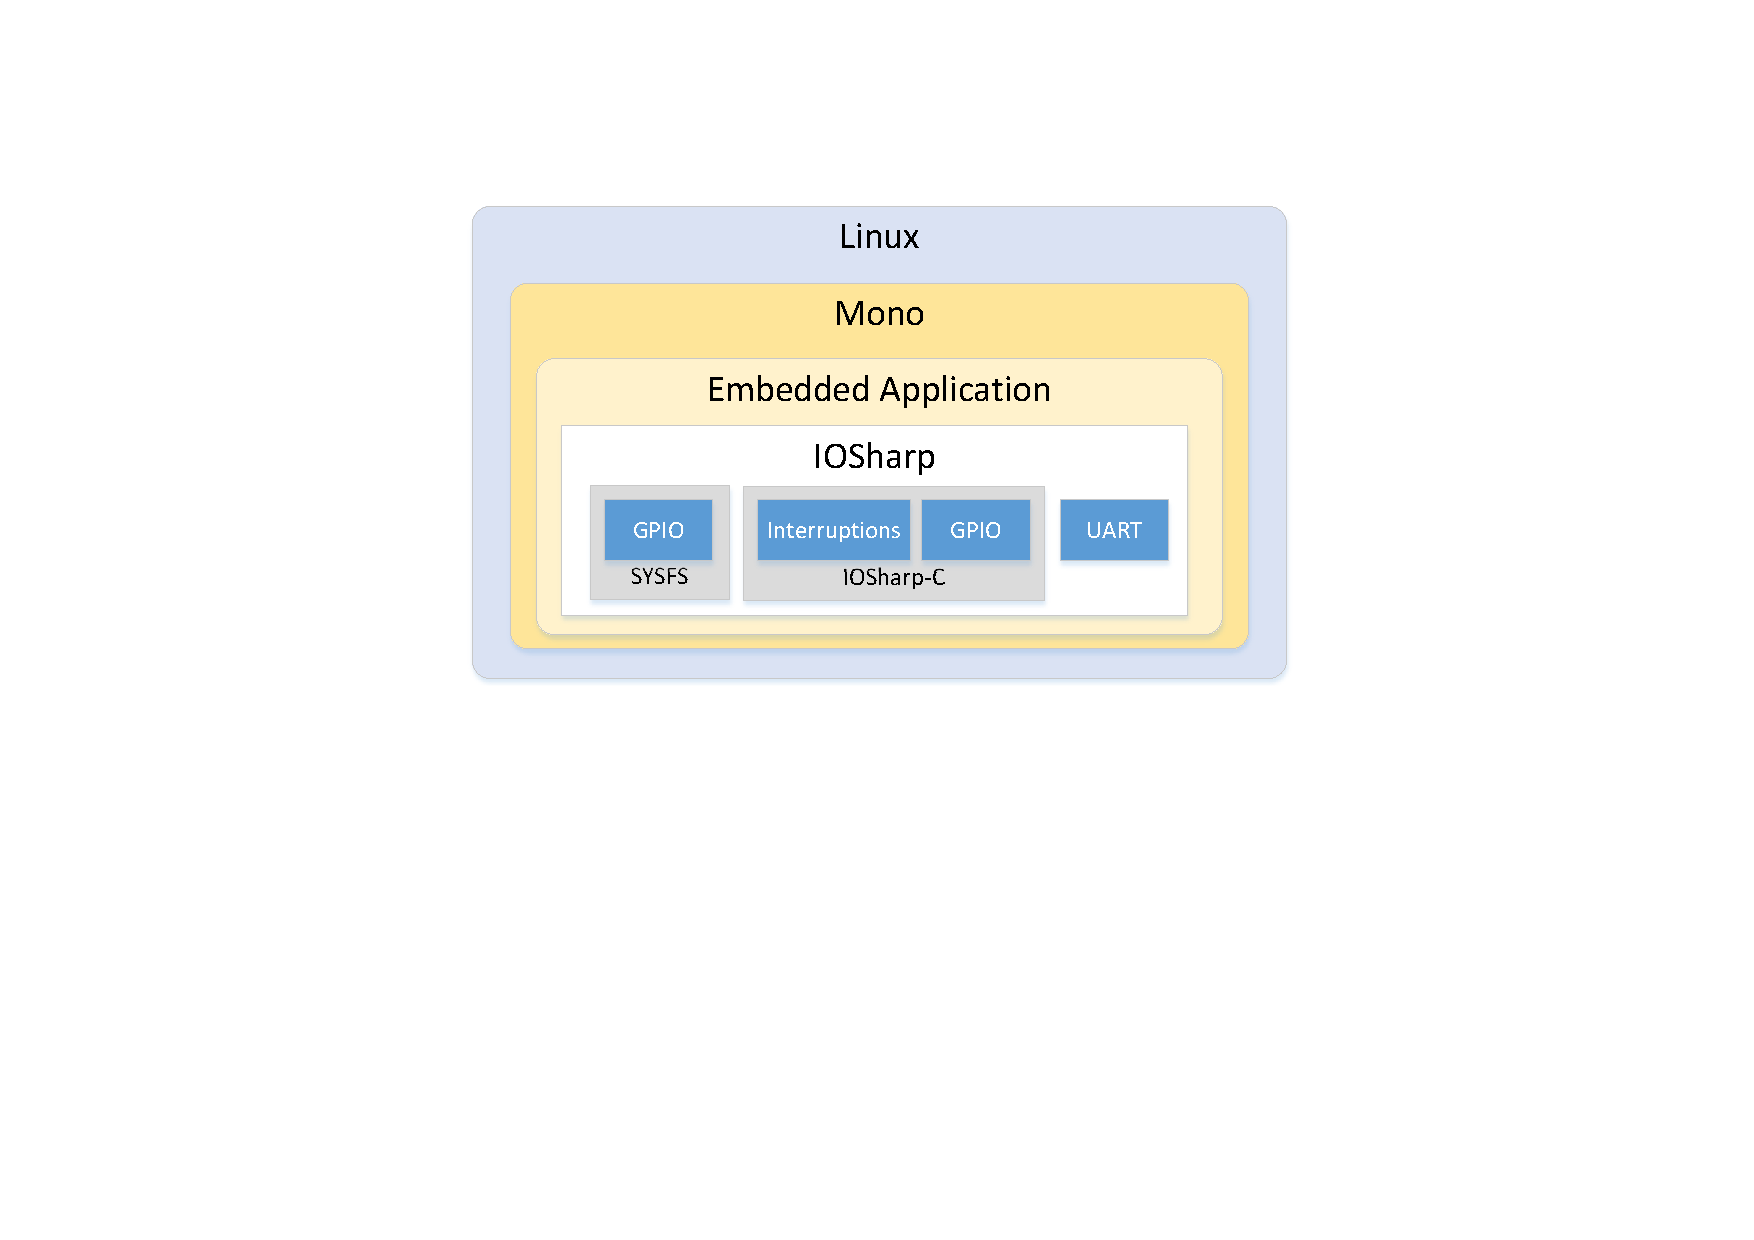
\includegraphics[scale=0.75]{pictures/iosharp/iosharp-schema2}
  \caption{Representation of the IOSharp \label{fig:interrupt-schema}}
\end{center}\end{figure}

\subsection{GPIO}\label{SS:GPIO}
GPIO acronym stands for General Purpose Input Output which are Ports on systems that are capable of generating an output or reading an input with a certain level of voltage. Normally embedded systems work at 3.3V, but low power devices can work at 2V.

\subsubsection{Implementation Options}\label{SSS:Implementation-Options}
In order to implement the GPIO ports in Micro Framework, it will be used the \verb!IOPorts.cs! file which contains the structure for Input, Output, Tristate and Interrupt ports. The first three will be explained in this section whereas the interrupt port will have a dedicated one.
\\
The GPIOs in Linux can be controlled in several ways. The most common and simple is to use the \gls{SYSFS}, which stands for a set of directories with readable and writeable files representing the ports of the CPU. On the other hand, the Linux kernel also provides a library to control the pins.
\\
The decision must be done between these two systems. In order to use any of this solutions the GPIO module must be loaded into the kernel. Many desktop Linux distributions have GPIOs disabled and that's why the kernel must be recompiled enabling this feature.
\\
In case of Linux operating systems designated for embedded devices, for example the Raspberry Pi or CubieBoard, they will have the I/O Ports enabled by default.
\\
It is interesting to point that Android is capable to use GPIO ports. Although it cannot seem an interesting feature nowadays, android is everywhere and can run in many devices, so this is another reason to try to fetch this sector in future versions of IOSharp.

\subsubsection{Using GPIO from SYSFS}\label{SSS:IOSharp-GPIO-SYSFS}
Since each solution can be used in this project and both are available in any Linux it was decided to use the SYSFS access because it is much easier to use and test the implementation. It only requires having read/write access to a certain set of files and directories and by reading or writing in this ones is possible to change the port states.
\\
\\
As it was said before, in SYSFS the control of the GPIOs is carried by several files and directories located under \verb!/sys/class/gpio! directory. In this directory there are two files which are called \verb!export! and \verb!unexport!, the first one is used to enable a GPIO while the second one disables it. After enabling a GPIO a new folder is created representing the enabled port, for instance if port 2 is enabled, a folder called gpio2 will be created. Inside this new folder there are several files, the \verb!direction! file describes how port should work, if the desired function is as an input port an \verb!in! must be written in the file whereas \verb!out! is used for an output port. After setting the port direction the next relevant file is \verb!value! which is used to set the port state in case of an Output Port (write 0 for a state-low or a 1 for a state-high) or in case of an Input Port it will read the incoming value through the port.

\subsubsection{Implementing in NETMF}\label{SSS:Implementing-GPIO-NETMF}
Taking in mind that this implementation has to be done over the existing code extracted from the \verb!IOPorts.cs! file, is important to design how to do it properly, in this case a \verb!GPIOManager! has been created using a singleton pattern. This class will restrict the number of instantiations that a port can have in order to avoid problems on the hardware. The instance of this singleton is shared across all the code.
\\
This manager will be in charge of enabling, disabling and operating the different I/O ports. Apart from this it also controls if a port is instantiated to avoid problems related to instantiate two port types in a unique pin.
\\
The figure \ref{fig:gpio-uml} shows the UML diagram of the \verb!IOPorts.cs! file from Micro Framework. Each class uses the \verb!GPIOManager! to control the read/write functions and port creation.

\begin{figure}[H]\begin{center}
 \centering
  \captionsetup{justification=centering}
  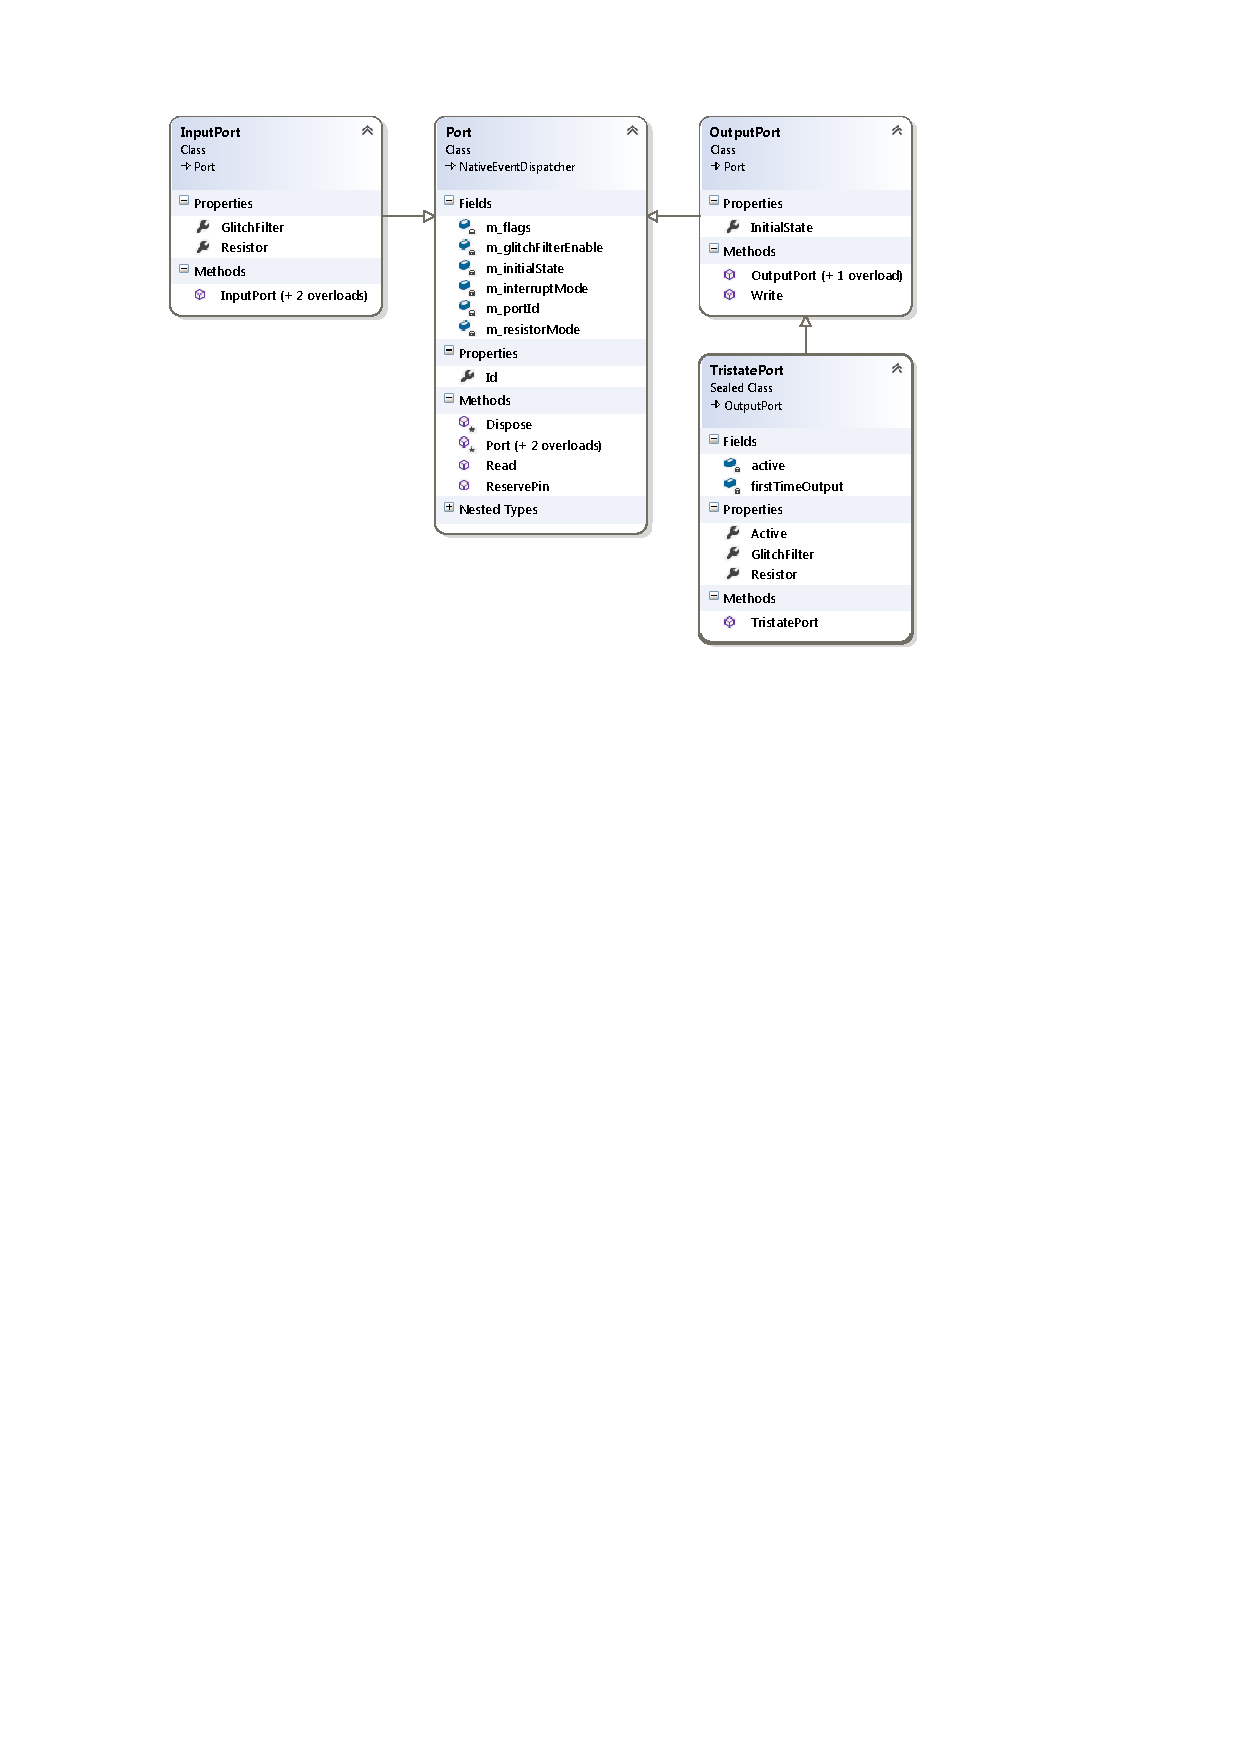
\includegraphics[width=1\textwidth]{pictures/iosharp/gpio}
  \caption{UML Diagram of NETMF Port and its inheritance \label{fig:gpio-uml}}
\end{center}\end{figure}

As is shown each port type inherits from the \verb!Port! object which implements the methods to enable or disable a port. \verb!Read! method is used to obtain the current state of the port i.e read an input value or even know the configured state in an output port. Finally the \verb!ReservePin! method permits to reserve a pin for a future usage.
\\
The \verb!InputPort! inherits from Port and it does not have any special method apart from its constructor which bases to the \verb!Port! class. 
\\
The \verb!OutputPort! which also inherits \verb!Port! implements a new \verb!Write! method which is used to write a state through the port (active-high or active-low).
\\
The \verb!TristatePort! inherits from \verb!OutputPort!. This port can change its functional work between an input or an output mode.

\subsection{Interruptions}\label{SS:IOSharp-Interrupt}
The interruptions which are needed for the interruptions that are required in the HomeSense program when using the \gls{SPI}. Although the \gls{BCM2835} supports native interruptions via \gls{IRQ} at the time of this project was developed the Raspberry Pi did not support GPIO interruptions using \gls{IRQ}.

\subsubsection{Designing the Interruptions}\label{SSS:IOSharp-Interrupt-Design}
The interruption system has been written in C in order to use a function called \verb!poll! which is commonly used by developers that want to detect GPIO interruptions using the SYSFS. The \verb!poll! function must be configured to wait and block until certain events occur on a \gls{FD} corresponding to a GPIO port enabled on the SYSFS. This function is configured to wait and block the program execution until the a \verb!POLLPRI! event on the \gls{FD} is detected. This event will be triggered by the OS when the file had urgent data to be read. Poll function will dectect the event and then will proceed with the following instructions to read different parameters from the port (i.e. the port state). Then, in C\# a delegate pattern will be used to notify to the upper layers of the program that interruption. The developer will configure the function which acts as the delegate by passing it to the \verb!OnInterrupt! property in the Interrupt Port.

\begin{figure}[H]\begin{center}
 \centering
  \captionsetup{justification=centering}
  \includegraphics[width=1\textwidth]{pictures/iosharp/interrupt-uml}
  \caption{UML Diagram of NETMF Interrupt Port \label{fig:interrupt-uml}}
\end{center}\end{figure}

\subsubsection{Platform Invocation Services}\label{SSS:IOSharp-Interrupt-PInvoke}
In C\# is possible to invoke external libraries which are not written in the same language. In this case, the library used for the interruptions is written in C and it will be compiled into a shared library making it available to any program, or in this case, IOSharp.
\\
\\
Take a look into the appendix \ref{S:appendices-libraries-types} to know more about the different library types.
\\
\\
P/Invokes in .NET make use of dynamic loaded libraries in order to use the contained functions. The implementation difficulty of a P/Invoke increases on how complex is the function to be called regarding its parameters, for basic type parameters such us \verb!int!, \verb!long!, \verb!byte! is really simple to make a P/Invoke call, but when passing object parameters things get much more difficult because this requires doing marshalling in this objects. Marshalling is similar to serializing but maintaining some information related to the object. The marshalling is used to pass from managed to unmanaged code and sometimes is impossible without using intermediate structs as interchange objects.
\\
\\
Below are shown the important parts of the implementation of this library and then how P/Invoke is done in C\# code.
\\
This first block shows the function which is used to detect the interruptions on the GPIOs. The interesting parts are commented explaining what they do or what some macros mean.
\begin{lstlisting}[language=C, caption={IOSharp.c - Polling function}]
uint64_t start_polling(int pin) {
    struct pollfd fdset;
    int nfds = 1;
    int gpio_fd, timeout, rc;
    char * buf[MAX_BUF], c;
    int len, count, i;
    long t;

    // Get the File Descriptor for the GPIO Port. See function on the Library.
    gpio_fd = gpio_fd_open(pin);

    // Clear any initial pending interrupts
    ioctl(gpio_fd, FIONREAD, & count);
    for (i = 0; i < count; ++i)
        read(gpio_fd, & c, 1);

    // Fill fdset which is a struct for pollfd which is used to describe the polling system.
    // In this case the File Descriptor for the GPIO port is entered, and then the POLLPRI (Data Urgent to Read) is configured as the event type.
    fdset.fd = gpio_fd;
    fdset.events = POLLPRI;

    read(fdset.fd, & buf, 64);

    // Start polling the File Descriptor. POLL_TIMEOUT variable contains (-1) which stands for infinite blocking until event.
    rc = poll( & fdset, 1, POLL_TIMEOUT);

    // Close the GPIO Port. See function on the Library.
    gpio_fd_close(gpio_fd);
    return t;
}
\end{lstlisting}
After writing the function this must be exposed using a header file which is shown below.
\begin{lstlisting}[language=C, caption={IOSharp.h - Header file for the library}]
#ifndef IOSHARP_H_INCLUDED
#define IOSHARP_H_INCLUDED

// Define the polling function
uint64_t start_polling(int pin);

#endif
\end{lstlisting}
And finally this block represents how is done a P/Invoke in a C\# program. The function is exposed using a \verb!public static extern! and then an attribute is attached which corresponds to the \verb!DllImport! which specifies the shared library to call.
\begin{lstlisting}[language=CSharp, caption={GPIOManager.cs - P/Invoke section}]
// The function which calls the external function
private void Listen(object obj) {
    ThreadHelper th = (ThreadHelper) obj;
    while (true) {
        int pin = (int) th.Pin;
        // Call the function. See down.
        ulong cback = GPIOManager.start_polling(pin);
        th.Callback(4, (uint) 0, DateTime.Now);
    }
}

// External function represents a function on an external library, in this case the library is the libIOSharp-c.so. The function naming and functions parameters are equal to the original function, but taking into account that a ulong in C# is a uint64_t on C.
[DllImport("libIOSharp-c.so", CallingConvention = CallingConvention.StdCall)]
public static extern ulong start_polling(int gpio);
\end{lstlisting}

\subsubsection{Final implementation}\label{SSS:IOSharp-Interrupt-Implementation}
The program flow is shown on Figure \ref{fig:interrupt-schema} which represents the steps that IOSharp does for the interruptions system. The Interrupt Port inherits from Input Port as Figure \ref{fig:interrupt-uml} shows.
\begin{figure}[H]\begin{center}
 \centering
  \captionsetup{justification=centering}
  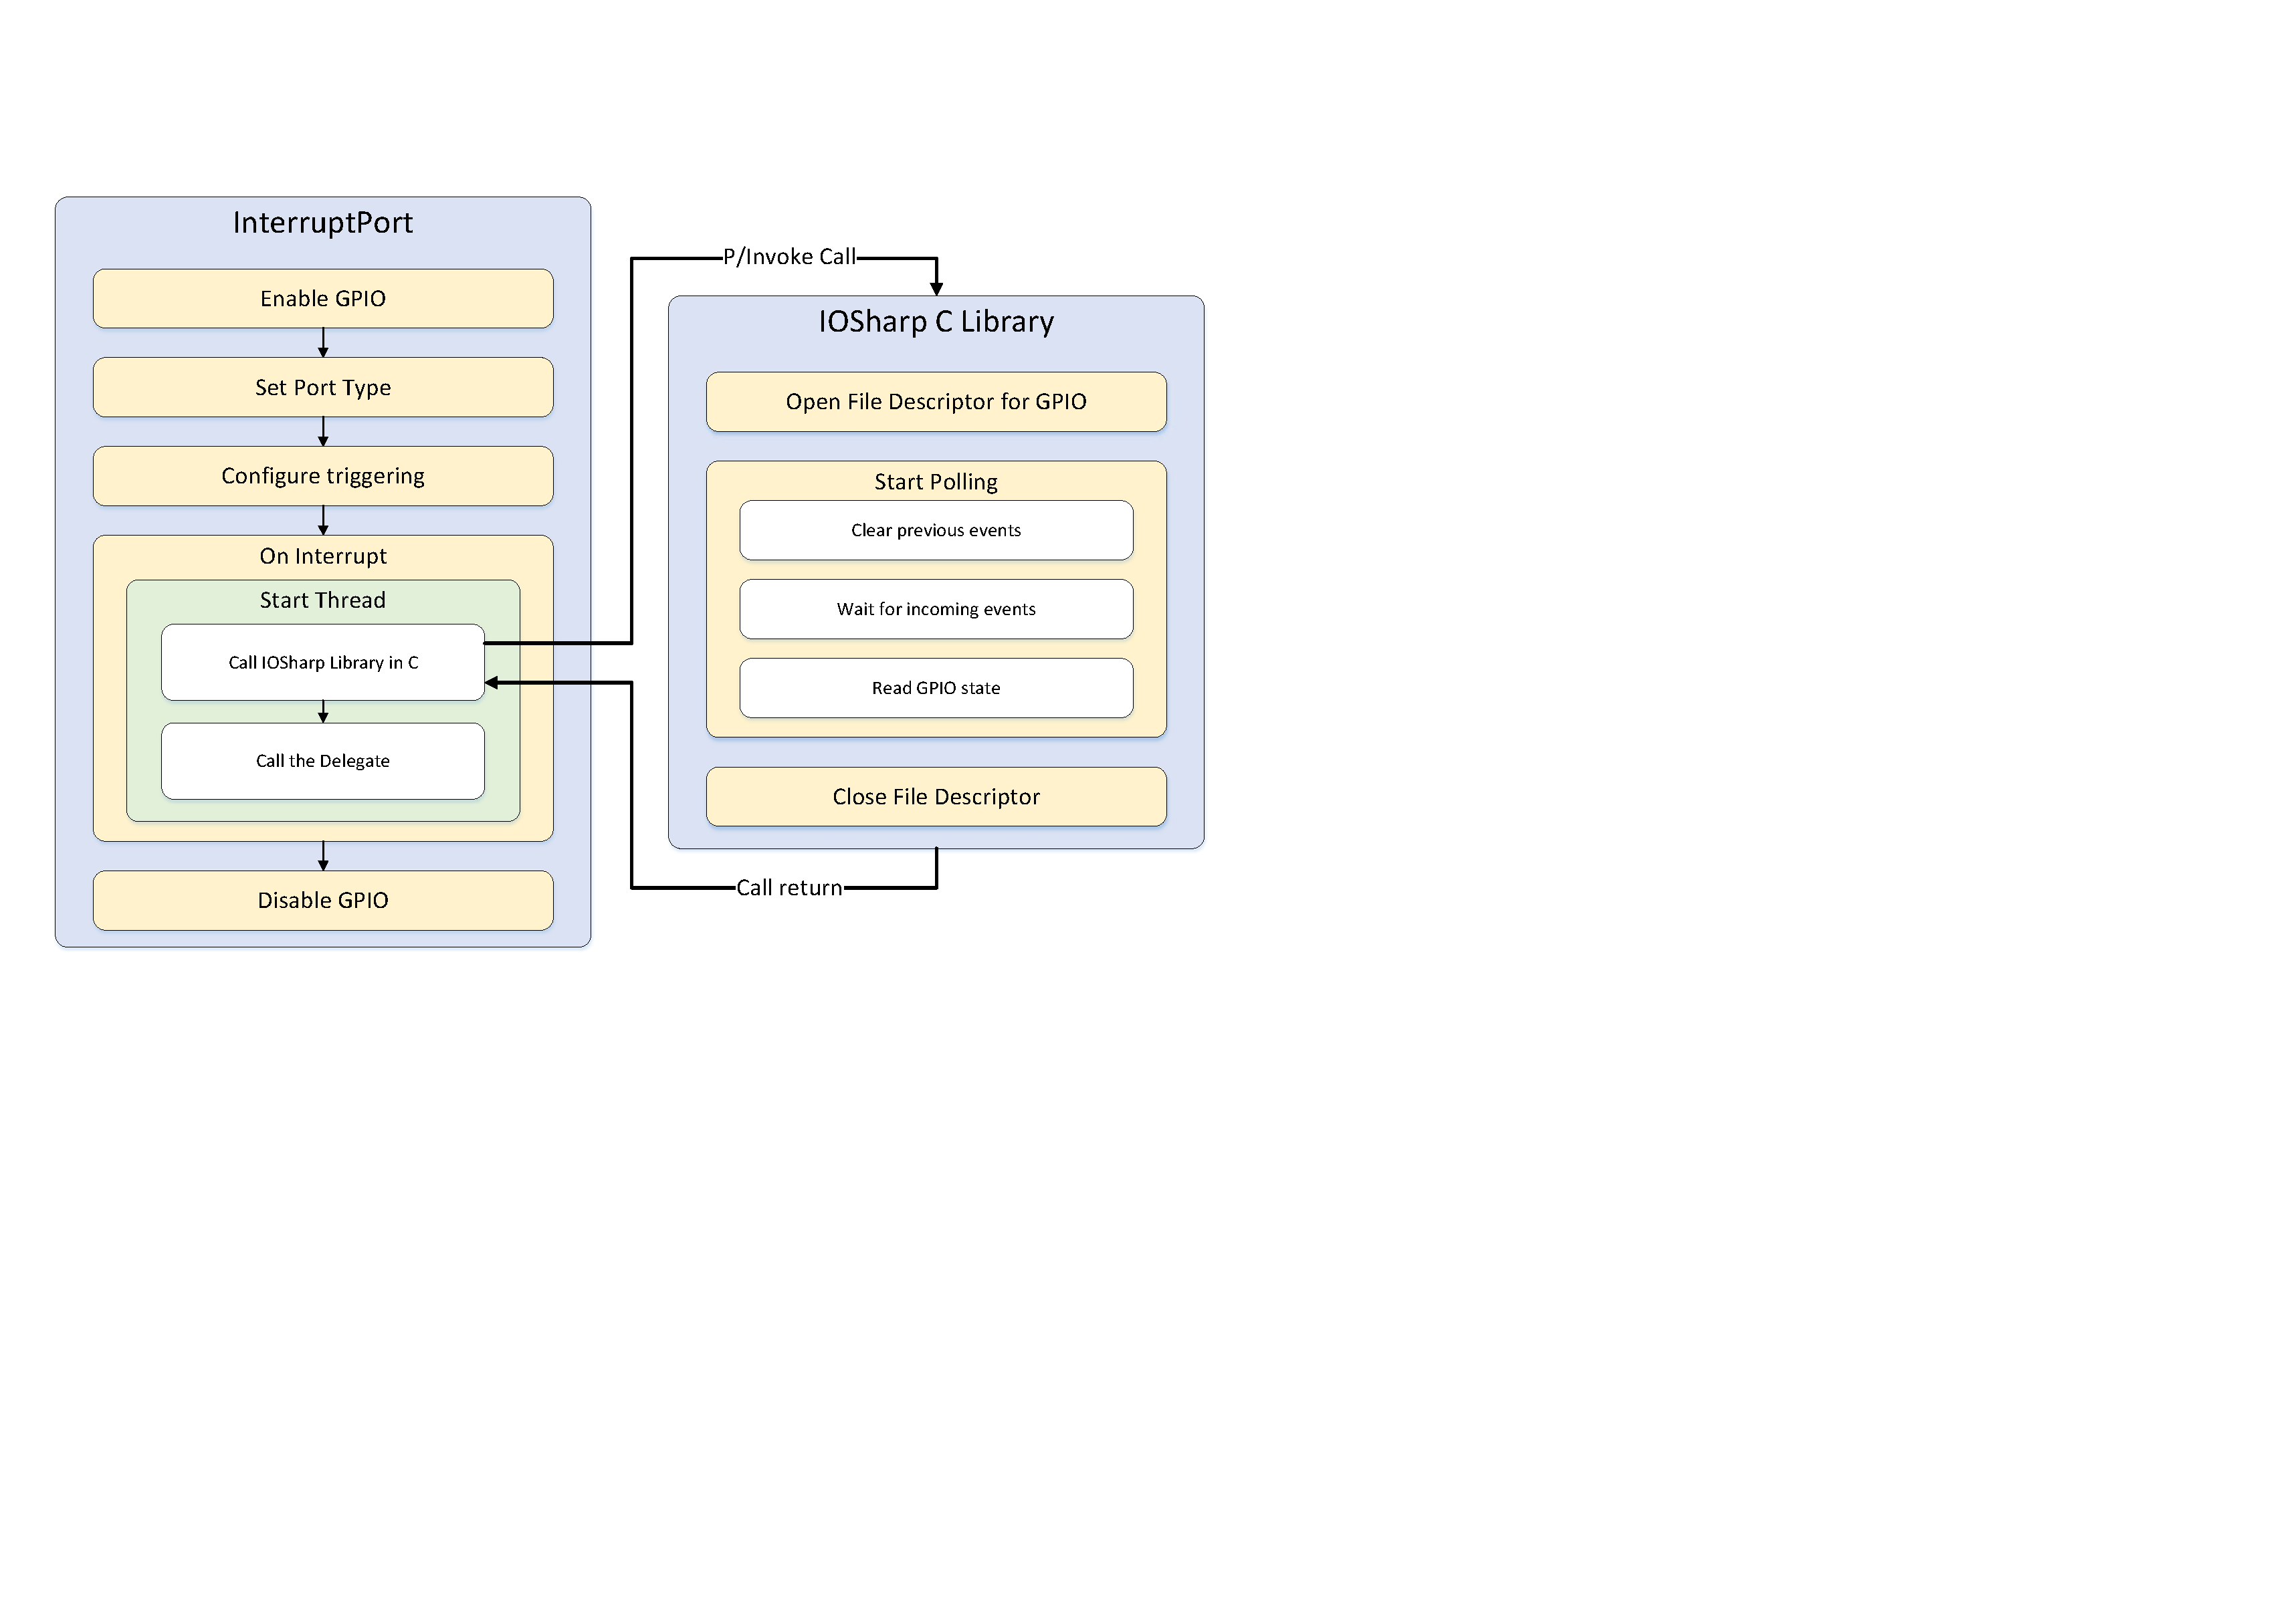
\includegraphics[width=1\textwidth]{pictures/iosharp/interrupt-schema}
  \caption{Representation of the Interrupt Port flow \label{fig:interrupt-schema}}
\end{center}\end{figure}
The idea is to do the exact same steps like the other ports do, the port enabling is done by the Port implementation which is the base class for Interrupt Port, then the port type is set to be an Interrupt Port, after doing this is the triggering must be configures. Micro Framework boards usually support four kinds of interruptions whereas Linux supports a few less, in the table \ref{T:Interrupt-Trigger-Types} are shown the ones that are supported. It is important to know that the edges are the point where the read state changes from one level to the other one. The Level is used when the state is maintained several time without changing.

\begin{table}[htb]
\begin{center}
\begin{tabular}{|c|c|c|}
\hline
{\bf Trigger Type} & {\bf Micro Framework} & {\bf Linux}  \\ \hline \hline
InterruptNone        & X    & X       \\ \hline
InterruptEdgeLow        & X    & X       \\ \hline
InterruptEdgeHigh        & X    & X       \\ \hline
InterruptEdgeBoth        & X    & X       \\ \hline
InterruptEdgeLevelHigh        & X    &        \\ \hline
InterruptEdgeLevelLow        & X    &        \\ \hline
\end{tabular}
\caption{Interrupt Trigger Types}
\label{T:Interrupt-Trigger-Types}
\end{center}
\end{table}

Like the GPIO the triggering is configured on the SYSFS on a file called \verb!edge! located inside of the enabled GPIO folder. This file can be configured on three different. \verb!EdgeLow! interruptions require the word \textit{falling} be written in that file, in case of \verb!EdgeHigh! \textit{rising} is used and finally \textit{both} is for \verb!EdgeBoth!.
\\
The polling thread works as an infinite loop P/Invoking to C and waiting for the call return, when this occurs the delegated function is called and this indicates that an interruption event occurred.

\subsection{SPI}\label{SS:IOSharp-SPI}
The \gls{SPI} is one of the important features to be implemented on IOSharp. This protocol is used in embedded systems to communicate boards and components in a Master-Slave way. It offers a full-duplex communication channel where the master and the slave can write and read at the same time. Normally this protocol accepts transmission frequencies in the range of 10 kHz to 100 MHz and in order to operate the master configures its clock using a frequency less or equal to the maximum frequency supported by the slave which wants to communicate.
\\
Figure \ref{fig:spi-modules} show how is used a SPI bus, a master device can have several slaves attached to its ports. The minimal system is composed by three ports which are the bus itself, the \gls{MOSI} is the channel where the Master device writes and from where Slaves read the written information. The \gls{MISO} is the channel where the Master reads the information that the Slave writes. The \gls{SCLK} is used to set the clock of the system between the Master and the Slave. Finally for each Slave it must be \gls{CS} in order to select the slave that must active during the transmission.
\begin{figure}[H]\begin{center}
 \centering
  \captionsetup{justification=centering}
  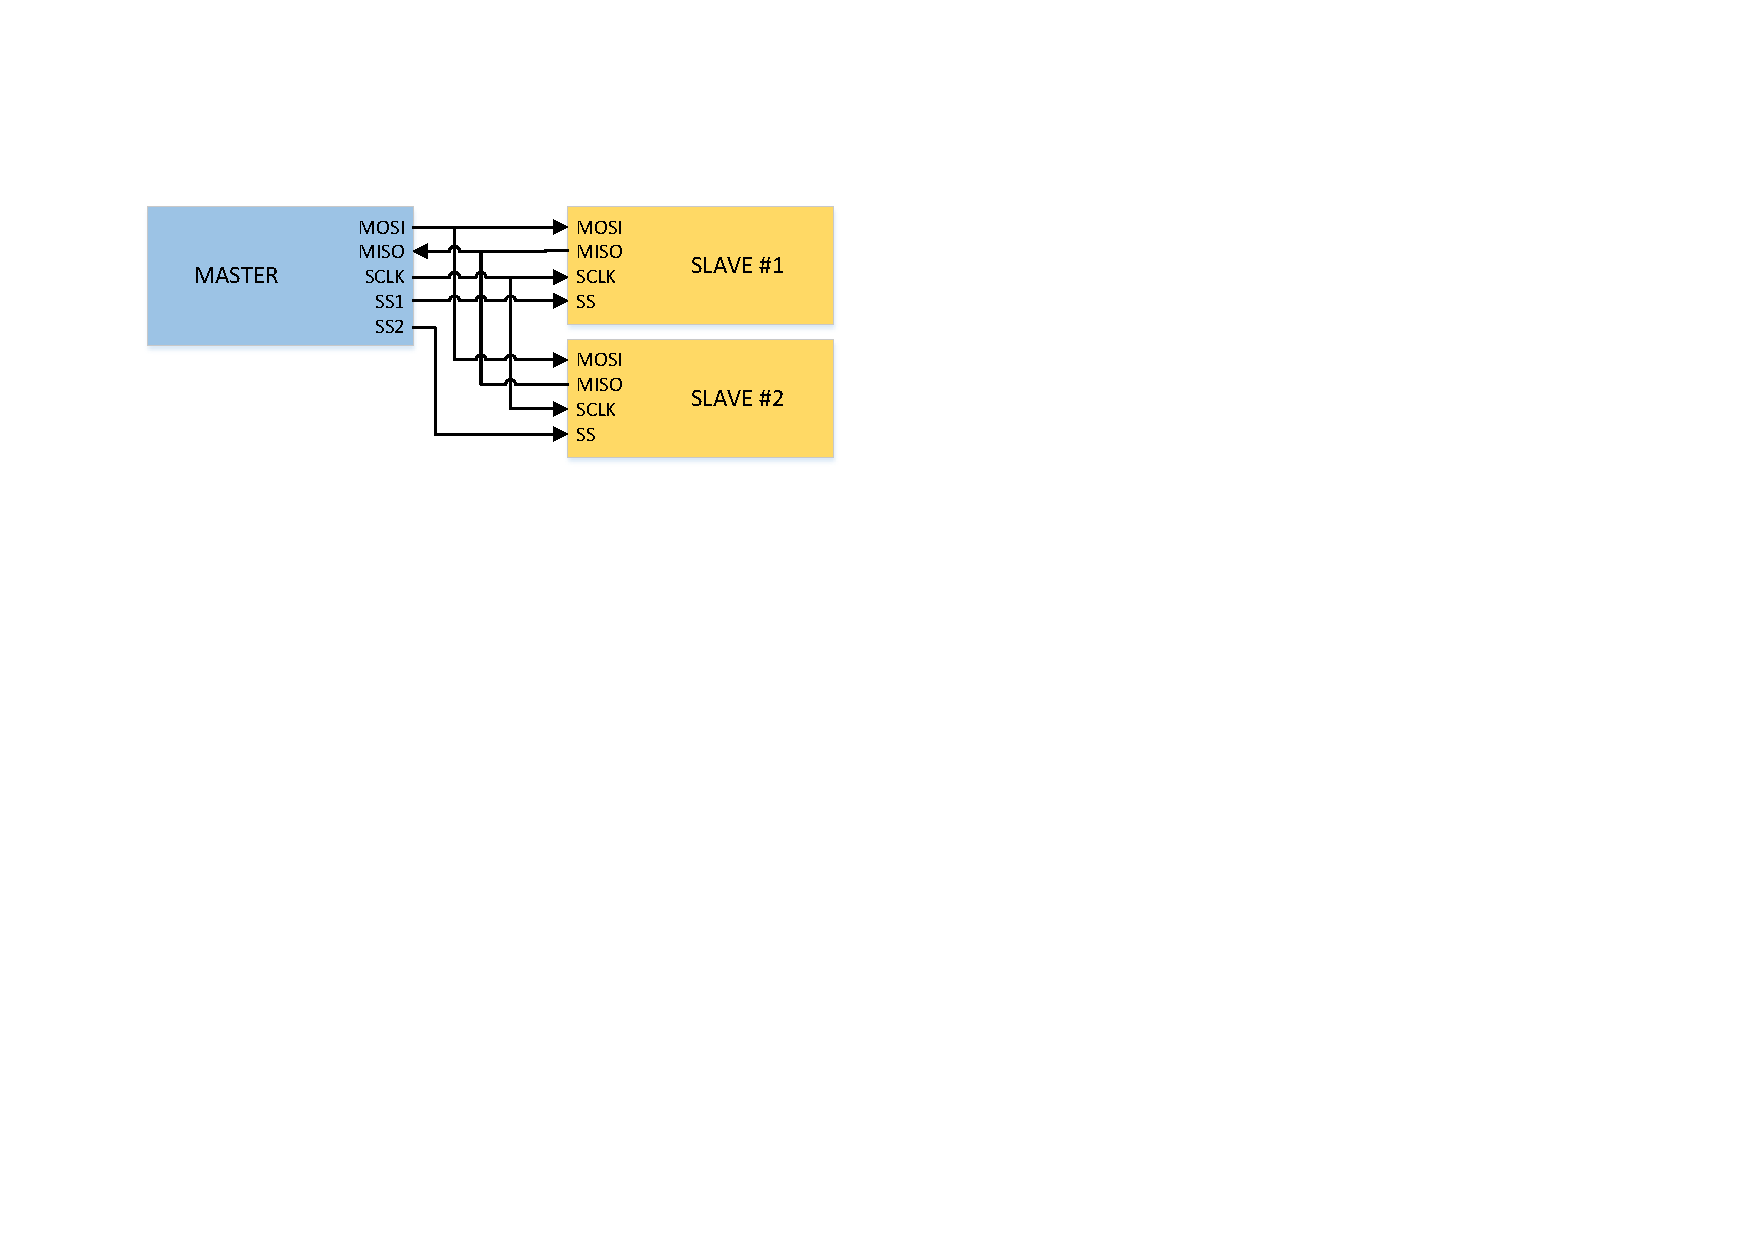
\includegraphics[scale=0.9]{pictures/iosharp/spi-modules}
  \caption{SPI bus setup with one master and two slaves \label{fig:spi-modules}}
\end{center}\end{figure}

\subsubsection{Designing the SPI}\label{SSS:IOSharp-SPI-Design}
The SPI implementation has been carried out like the Interrupt Port explained in the section \ref{SS:IOSharp-Interrupt}. In this case it has been used the Linux Kernel by using the \verb!<linux/spi/spidev.h>! library which makes the control of a SPI device very easy.
\\
SPI devices are mapped under \verb!/dev/! directory with a naming like \verb!/dev/spidevX.Y! the \verb!X! is an integer and represents the device (a CPU can have multiple SPI devices so this number will indicate the device number), then the \verb!Y!, also an integer, enumerates the \gls{CS} (SPI devices have multiple chip selects, so they can have more than one slave).
\\
\\
Before doing a transaction via the SPI this must be configured, first of all defining the operational mode. Modes are defined with the parameters Clock Polarity (CPOL) and Clock Phase (CPHA). Both are related to the sampling edge according to the clock (SCLK) used in the communication. The CPOL defines the polarity of the clock so the sampling will be done when de clock is in edge low or in edge high according to the configured parameter, CPHA defines in which phase the sample must be done. This concept is much easy to understand using the figure \ref{fig:spi-modes} which shows the different CPHA and CPOL options with the equivalent SPI modes required to be configured in the C library.

\begin{figure}[H]\begin{center}
 \centering
  \captionsetup{justification=centering}
  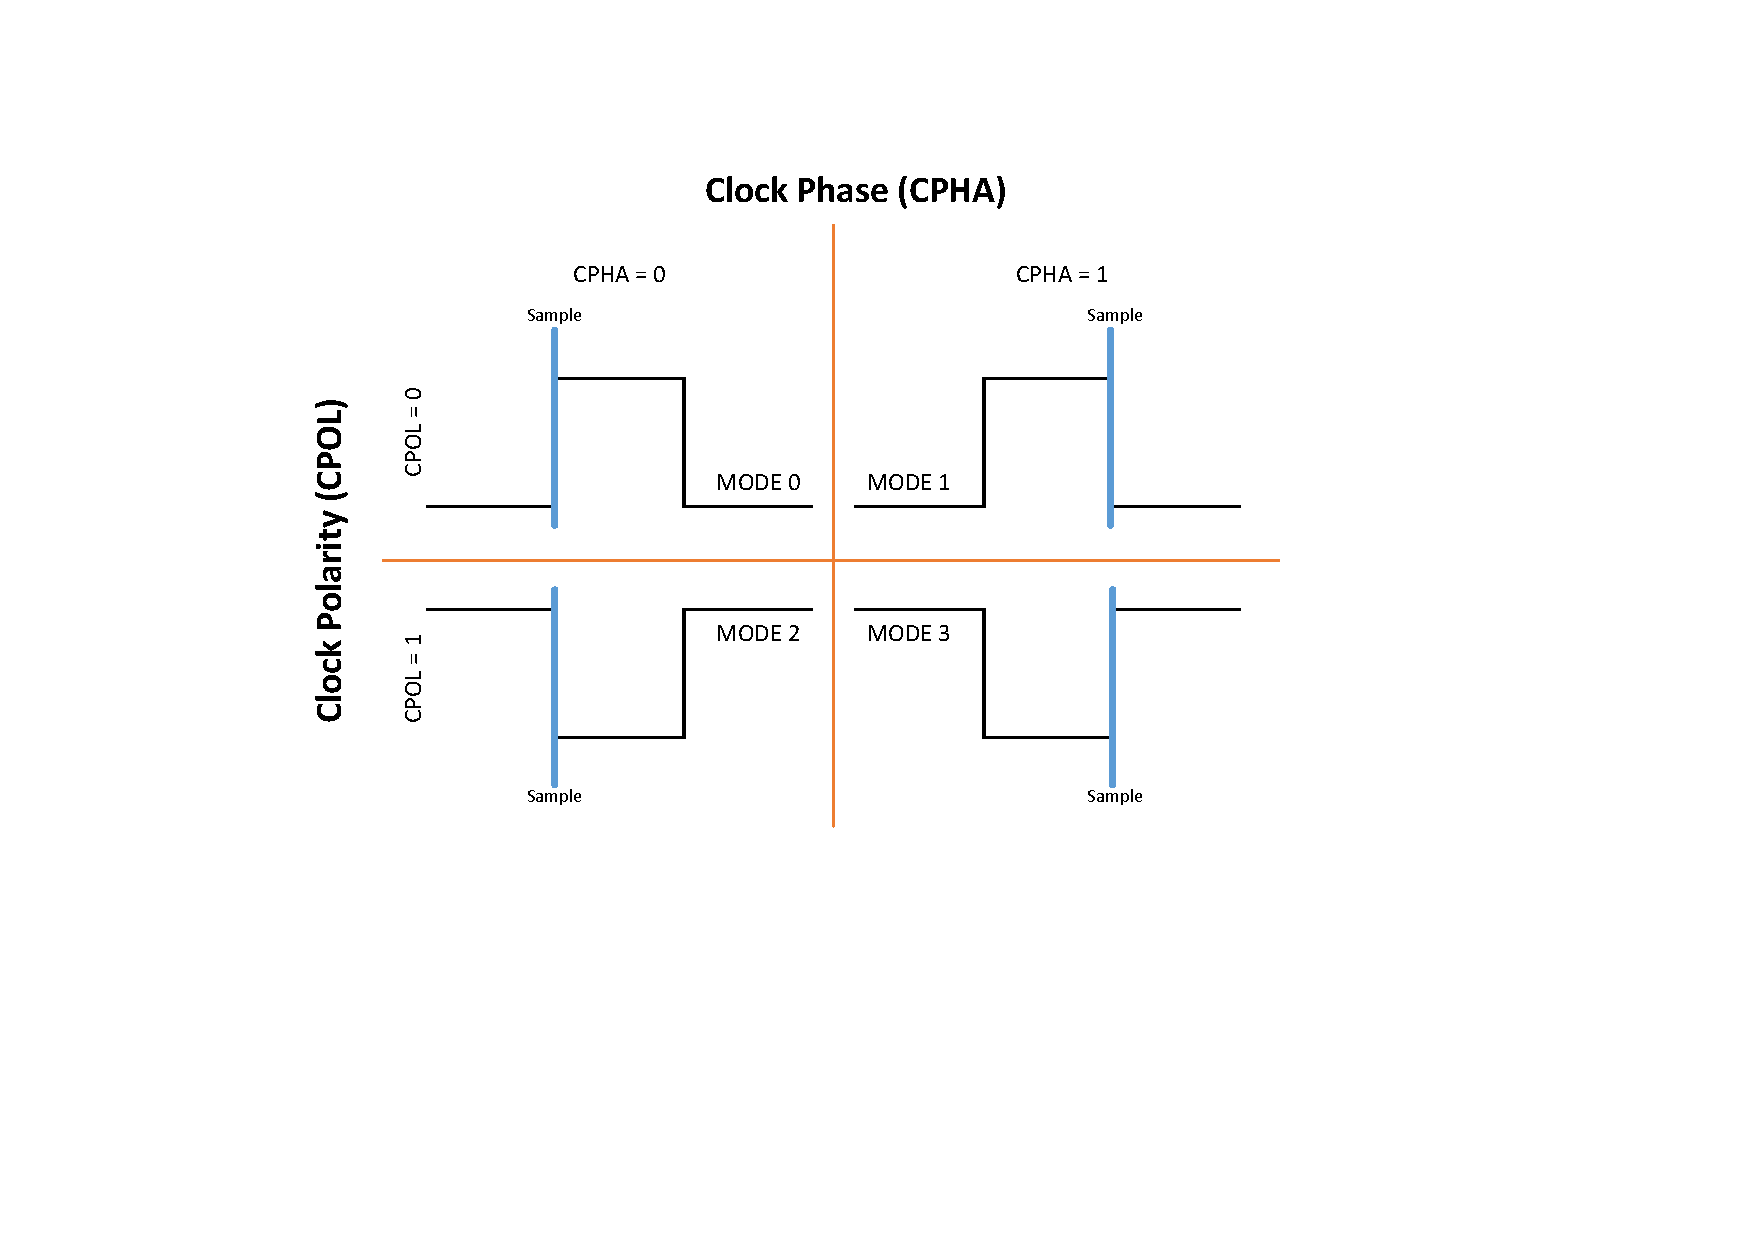
\includegraphics[scale=0.7]{pictures/iosharp/spi-modes}
  \caption{SPI modes are defined with the parameters "CPOL" and "CPHA" relatives to the data sampling acording to the System Clock (SCLK) state.\label{fig:spi-modes}}
\end{center}\end{figure}

This modes must be configured using the \gls{IOCTL} function passing the \gls{FD} according to the SPI device and the desired \gls{CS}, then the preprocessor macro \verb!SPI_IOC_WR_MODE! is used to specify which parameter will be configured, in this case its the SPI mode that has been explained before, the last parameter corresponds to another macro which defines the operational mode, the figure \ref{fig:spi-modes} shows each mode and the macro that must be passed to the \gls{IOCTL} function, this modes are \verb!SPI_MODE_0!, \verb!SPI_MODE_1!, \verb!SPI_MODE_2! and \verb!SPI_MODE_3!.

\begin{lstlisting}[language=C, caption={IOSharp.c - SPI Mode configuration}]
uint8_t mode;
  int ret;

//The mode variable can be SPI_MODE_0, SPI_MODE_1, SPI_MODE_2 and  SPI_MODE_3
  ret = ioctl(fd, SPI_IOC_WR_MODE, &mode);
  if (ret == -1)
    pabort("can't set spi mode");
\end{lstlisting}

Once the SPI mode has been configured a struct defining the transaction must be filled, the struct type of is \verb!spi_ioc_transfer! specified in the \verb!spidev.h! library. This struct contains different variables, the \verb!tx_buf! and \verb!rx_buf! are configured with the write and read. Apart from the buffers, the transmission length is configured using the variable \verb!len!. Then the delay is configured, this indicates how many microseconds the SPI driver must wait before starting the transmission, this is important because some slaves take some time between they are selected and they are able to communicate, this is configured using the \verb!delay_usecs! variable. Another parameter to configure is the clock by using \verb!speed_hz!. In order to deselect a device before a transfer, the parameter \verb!cs_change! must be true. Finally, to configure or override the wordsize of a transmission the\verb!bits_per_word! is used.

\begin{lstlisting}[language=C, caption={IOSharp.c - SPI struct configuration}]
struct spi_ioc_transfer tr = {
    .tx_buf = (unsigned long)writeBuffer,
    .rx_buf = (unsigned long)readBuffer,
    .len = writeCount,
    .delay_usecs = spi.delay,
    .speed_hz = spi.speed,
    .cs_change = spi.cs_change,
    .bits_per_word = 8,
  };
\end{lstlisting}

Once the struct is configured another ioctl call is done which makes the transfer it self. In this case, along with the \gls{FD} corresponding to the SPI device another preprocessor macro is passed as a parameter, this one is called \verb!SPI_IOC_MESSAGE! and must include the number of transfers that will be executed together, in case of IOSharp there is only one transfer per call, so the parameter will look like \verb!SPI_IOC_MESSAGE(1)!, finally the struct commented above is included in the ioctl call.

\begin{lstlisting}[language=C, caption={IOSharp.c - SPI transfer}]
// Pass the preprocessor macro and the spi_ioc_transfer struct.
ioctl(fd, SPI_IOC_MESSAGE(1), &tr);
\end{lstlisting}

\subsubsection{Implementation in C\#}\label{SSS:IOSharp-SPI-Implementation-CSharp}
After writing the library part in C is time to modify IOSharp to add the necessary calls to this library in order to make Micro Framework use the SPI in Linux. In this case the calls will be done in a similar way as it has been done in the interruptions (\ref{SS:IOSharp-Interrupt}). In this case some data will need to be serialized in order to pass the configuration of the SPI from C\# to C.
\\
Essentially the method will be do a P/Invoke from C\# in order to call the functions in the library. To facilitate the data exchange between the program and the library a struct is used, this contains the basic information in order to do the configurations explained on the previous section. This struct must be written in the header file of the library and also must be written in the C\# code. First of all the SPI implementation in Micro Framework is divided into two blocks, the first one represents the port configuration which is used to set the different properties that can be used with the SPI, for example the clock rate, the setup time of the slave, the SPI modes (CPHA and CPOL), etc. The second block, which is the SPI itself uses the configuration commented above to create an SPI instance, along with the required pins for the \gls{MISO}, \gls{MOSI}, \gls{SCLK} and \gls{CS}.
\\
When the SPI instance is created, the methods will be able to be used, basically there are different overloads of the \verb!Write! and \verb!WriteRead! methods, but all of them end calling the same internal function which will do the P/Invoke to the library.

\begin{figure}[H]\begin{center}
 \centering
  \captionsetup{justification=centering}
  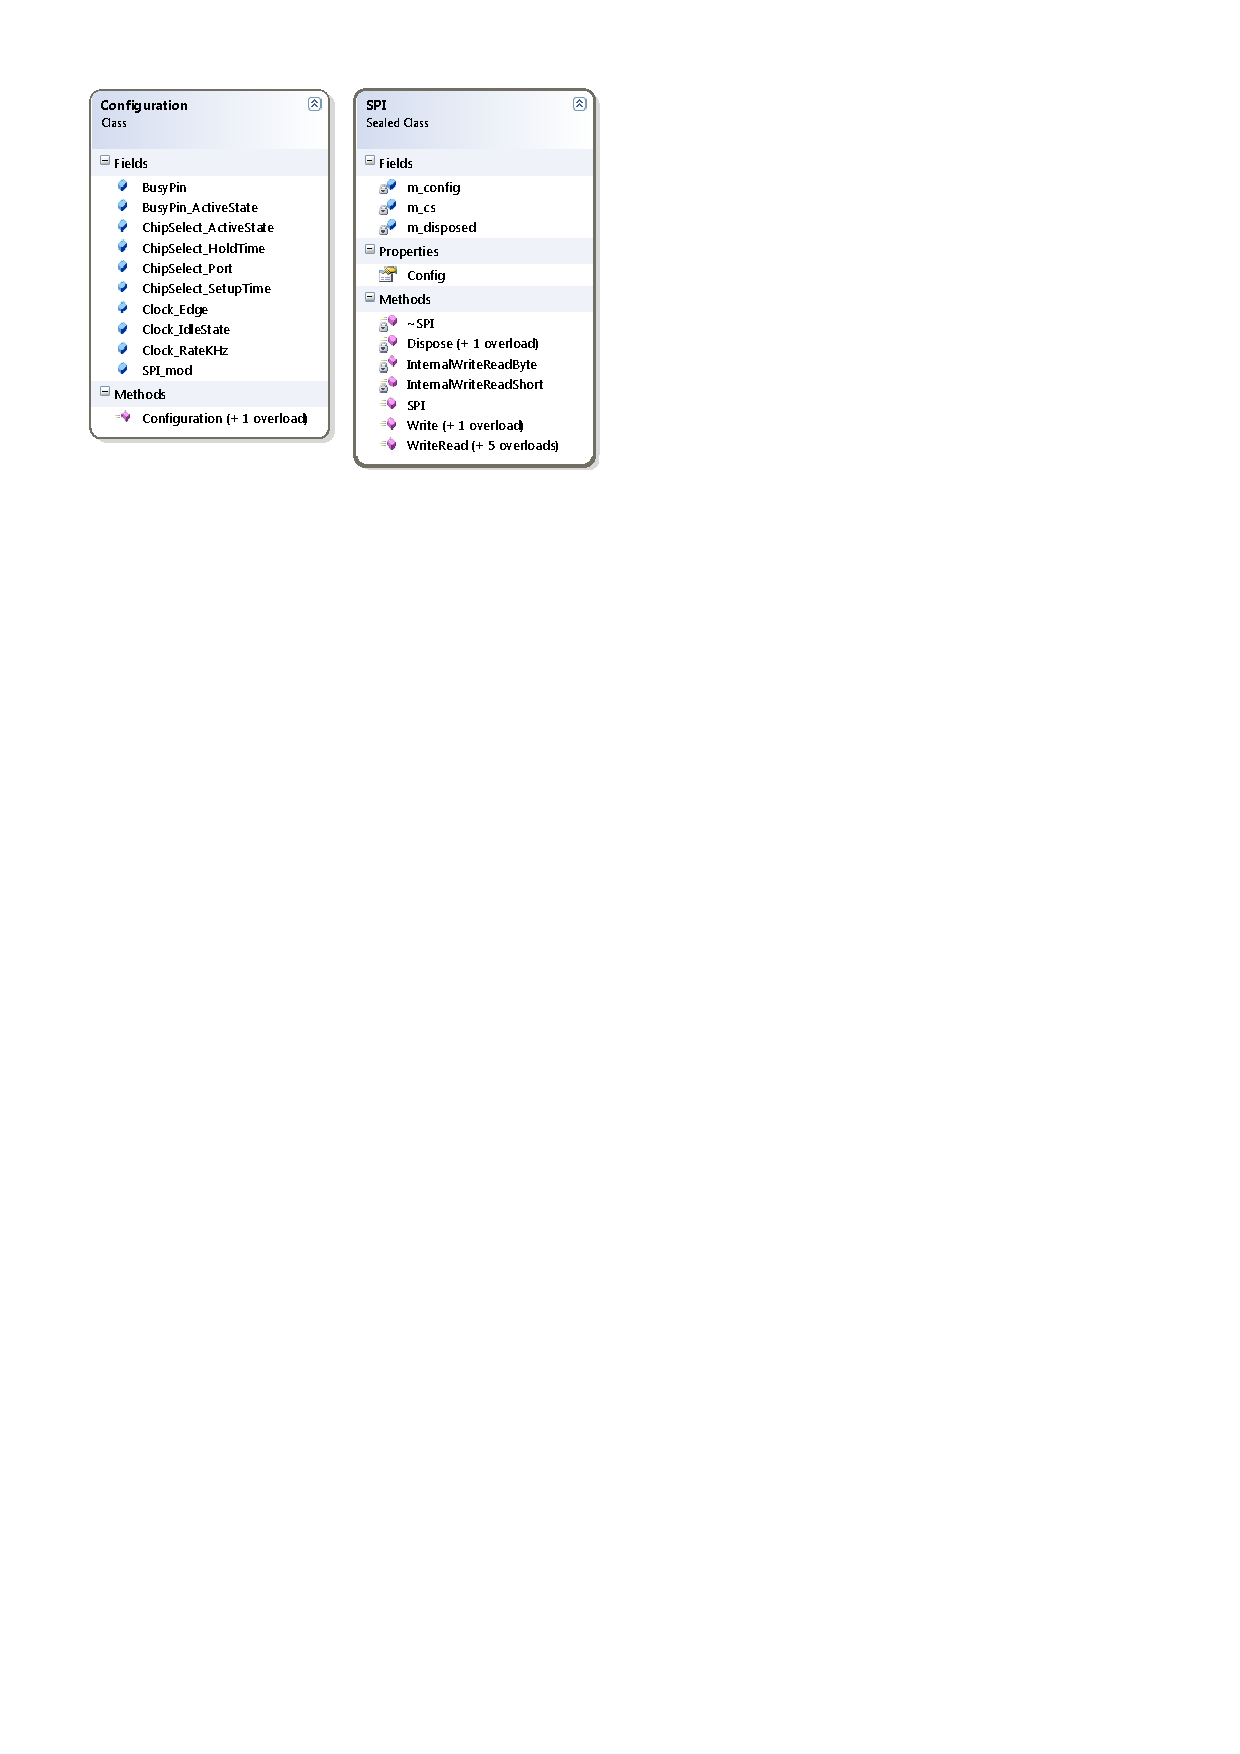
\includegraphics[scale=1]{pictures/iosharp/spi-uml}
  \caption{UML representation of the SPI Configuration Class (Left) and the SPI Port (Right) \label{fig:spi-uml}}
\end{center}\end{figure}

In order to pass the configuration to the library, the configuration object is converted to a struct which its variables are the same as the struct from the header file of the library. This struct will be the one that is passed to the C library.
\\
The code shown below corresponds to the header file and represents the struct that will be interchanged between the two languages.

\begin{lstlisting}[language=C, caption={IOSharp.h - spi\_config struct}]
typedef struct spi_config
{
  int mode;
  uint32_t speed;
  int cs_change;
  uint16_t delay;
} SPI_CONFIG;
\end{lstlisting}

The listing below represents the C\# implementation of the C struct used for the pin configuration, it contains the same parameters as the C version and also implements a constructor which simplifies the conversion between the Configuration class and this structure, the important thing in this case is the
\\
\verb![StructLayout(LayoutKind.Sequential, CharSet = CharSet.Unicode)]!. This attribute is used by the P/Invoke to know how the marshalling must be done when is passed to the library.

\begin{lstlisting}[language=CSharp, caption={SPI.cs - spi\_config struct}]
[StructLayout(LayoutKind.Sequential, CharSet = CharSet.Unicode)]
public struct spi_config {
    public int mode;
    public uint speed;
    public int cs_change;
    public ushort delay;

    public spi_config(Configuration config) {
        this.cs_change = (config.ChipSelect_ActiveState) ? 1 : 0;
        this.delay = (ushort) config.ChipSelect_HoldTime;

        if (config.Clock_Edge && !config.Clock_IdleState)
            this.mode = 0;
        else if (!config.Clock_Edge && !config.Clock_IdleState)
            this.mode = 1;
        else if (config.Clock_Edge && config.Clock_IdleState)
            this.mode = 2;
        else
            this.mode = 3;
        this.speed = config.Clock_RateKHz * 1000;
    }
}
\end{lstlisting}

It is interesting to remark that the \gls{TX}/\gls{RX} buffers are not returned from C to C\# but the buffers have been read and written so C takes the pointer of that buffer, which is the same as the C\# and then writes or reads the information from there. 

\subsection{UART}\label{SS:IOSharp-UART}
UART is a really simple protocol that uses an asynchronous serial communication between two devices. As figure \ref{fig:uart-modules} shows, each device have two ports which are the \gls{TX} for transmissions and \gls{RX} for receptions. The transmission port must be connected to the reception port on the other device. Both devices must share the ground.

\begin{figure}[H]\begin{center}
 \centering
  \captionsetup{justification=centering}
  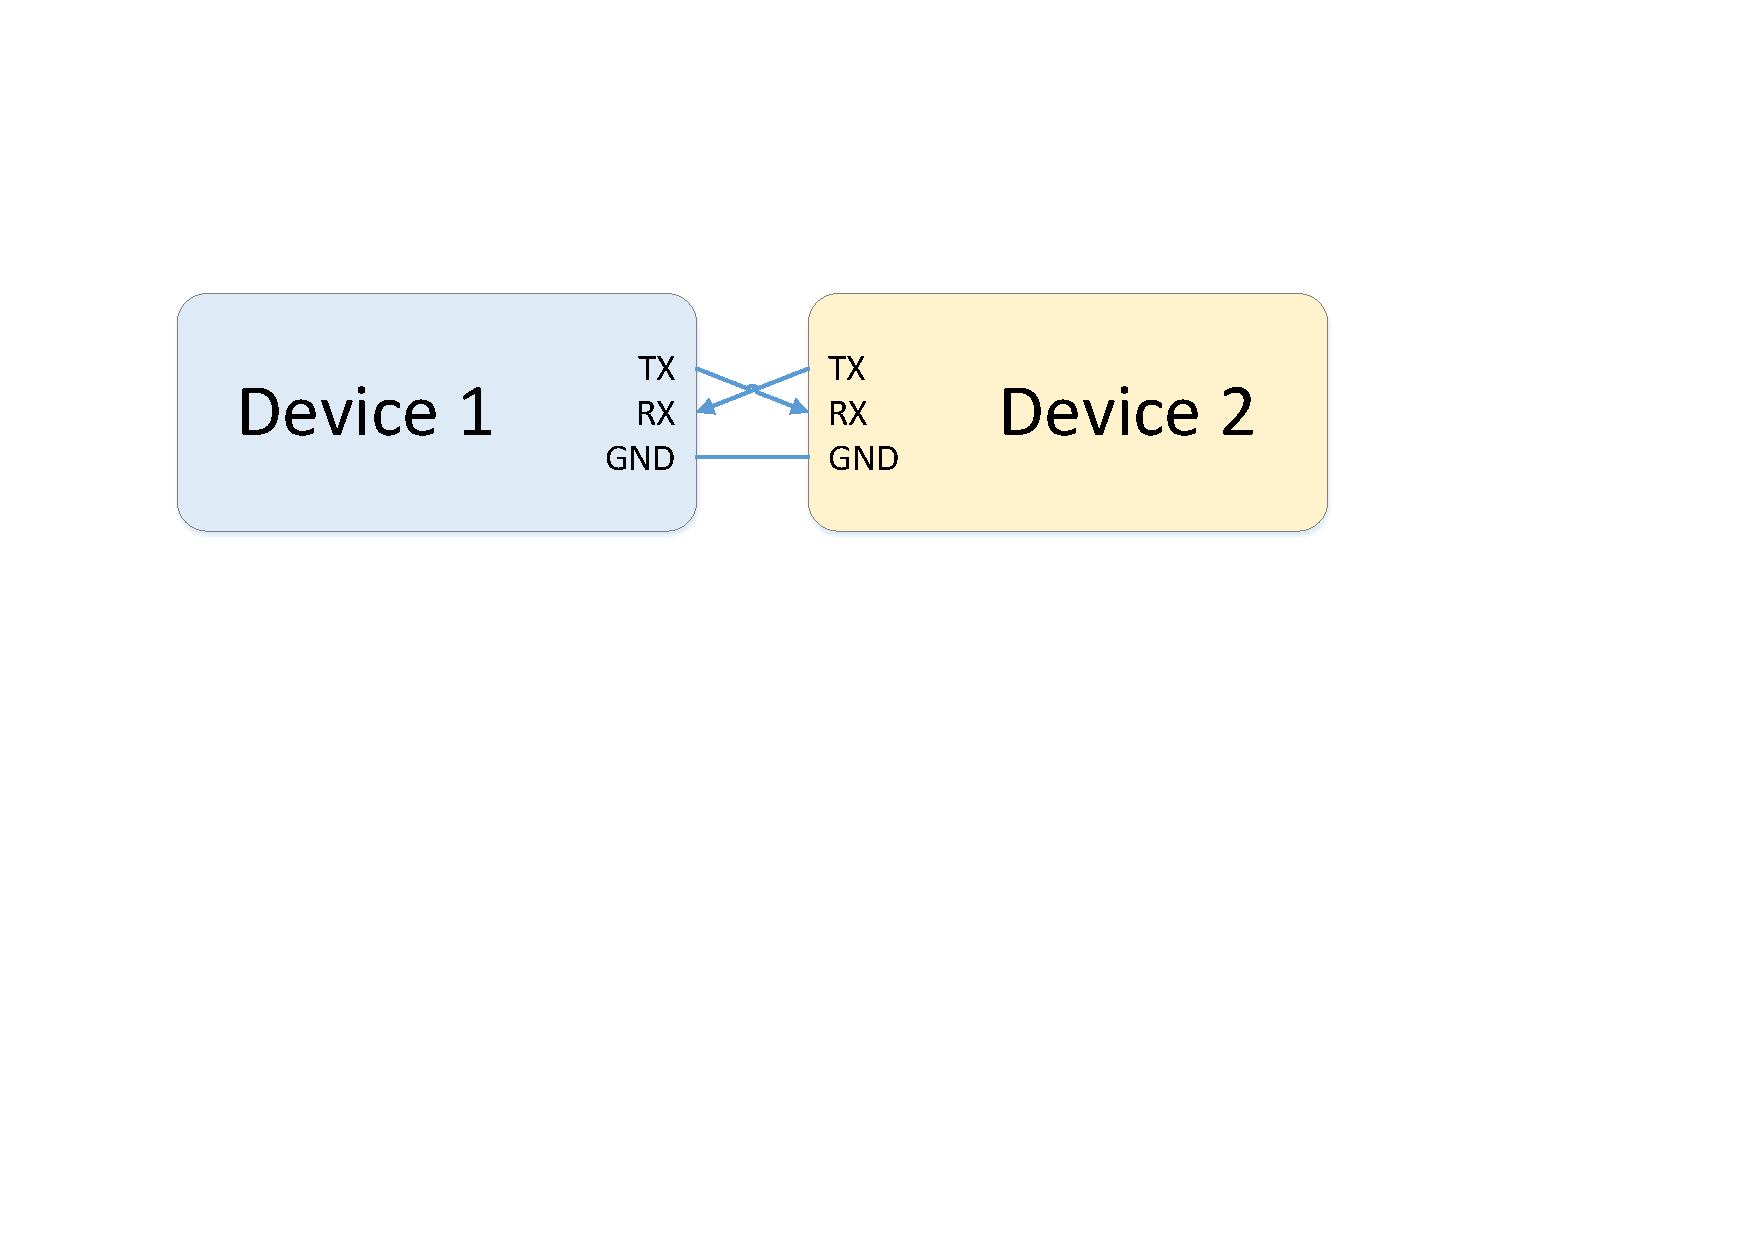
\includegraphics[scale=0.60]{pictures/iosharp/uart-modules}
  \caption{UART communication schema\label{fig:uart-modules}}
\end{center}\end{figure}

Unlike the above features which were not implemented on the standard .NET Framework the UART it is with also the same name and in the namespace, so this is problematic in case of a class reimplementation if maintaining the original namespace is desired.
\\
First of all and trying to avoid a new implementation of a SerialPort the classes from the Micro Framework and the .NET Framework were compared. After doing this it was realised that the two classes were so similar that IOSharp did not require a new reimplementation. The reason of avoiding a new implementation is due to two reasons, the first one is that any reuse of code is better rather than writing again the same feature, and considering that the communications between devices must be really well done, and .NET Framework is much more stable and tested than a code written from scratch. The other reason of this choose is that although the .NET Framework class is not exactly as the Micro Framework class, it has all the required methods that are needed for HomeSense.

\begin{figure}[H]\begin{center}
 \centering
  \captionsetup{justification=centering}
  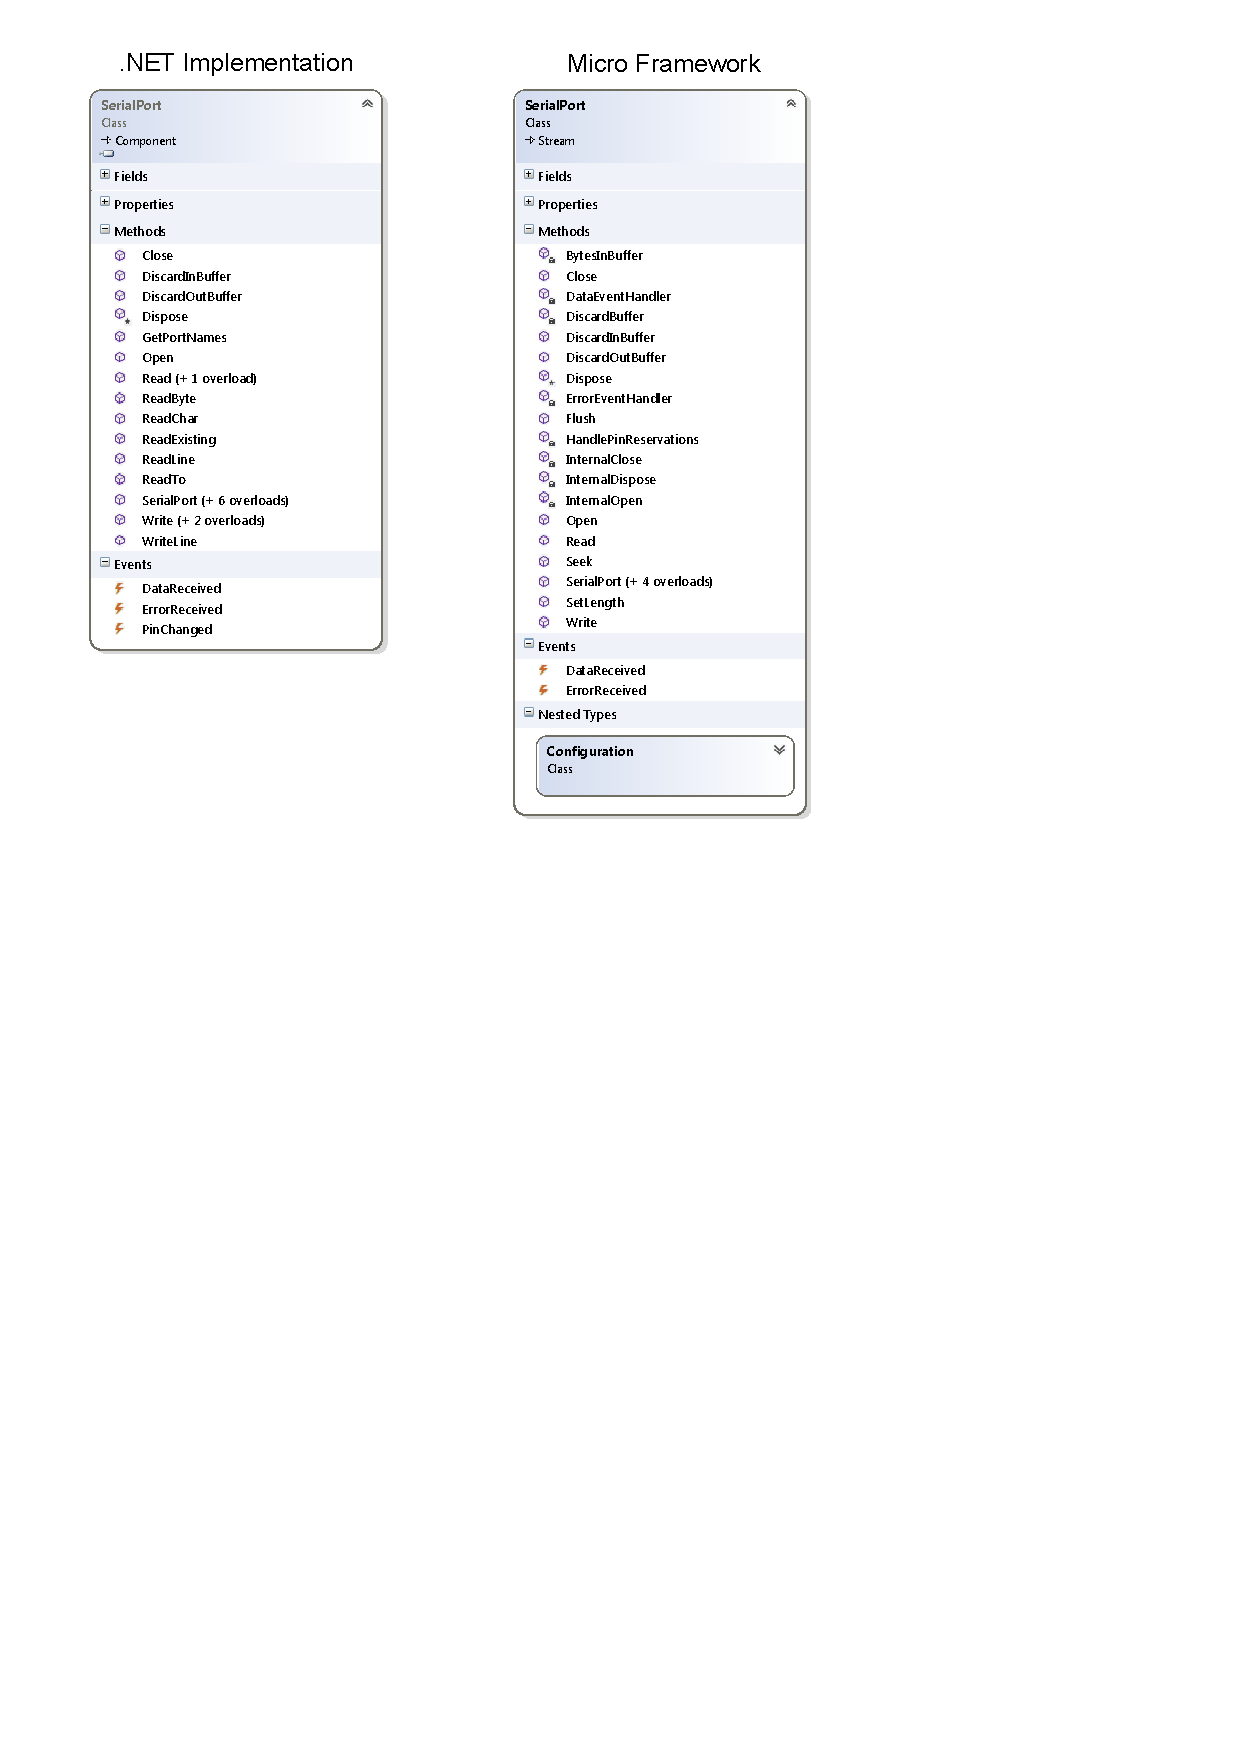
\includegraphics[scale=1]{pictures/iosharp/serialport-uml}
  \caption{UML SerialPort representation of the original .NET Framework (Left) and .NET Micro Framework (Right)\label{fig:serialport-uml}}
\end{center}\end{figure}

Is important to remark that IOSharp in Linux runs on Mono implementation of the .NET Framework classes, and in this case the SerialPort class has some disadvantages on Mono version, basically it does not support the \verb!DataReceived! or \verb!ErrorReceived! events because the functions have not been implemented on its internal runtime.

\section{Port Mapping}\label{S:Port-Mapping}
Although IOSharp is a cross-platform library some features require a specific configuration when deploying in different boards. Every board has its own port mapping and naming so it is necessary to have a specific library to describe that board.
\\
This is similar to the \gls{HAL} and \gls{PAL} concept:
\begin{itemize}
\item \textbf{HAL:} Hardware Abstraction Layer. In this case Linux acts as a HAL offering simple APIs to use features likes the kernel driven SPI device or the GPIO exposed in the SYSFS.
\item \textbf{PAL:} Platform Abstraction Layer. Is the library that must be implemented in order to exploit the HAL functionalities. In this case, the Raspberry Pi requires a library to remap the GPIO pins or the SPI device to the name that the HAL uses.
\end{itemize}

\subsection{HardwareProvider}\label{SS:HardwareProvider}
In fact, the original Micro Framework supports a hardware descriptor which represents the \gls{PAL} of the Raspberry Pi and is called \verb!HardwareProvider!. Raspberry Pi is the target platform for this project so a hardware descriptor was written, below are represented the pins of the Raspberry Pi, on the left the revision 1.0 and on the right the revision 2.0. In the image are also shown where are the different pins used for the SPI and the \gls{I2C}.

\begin{figure}[H]\begin{center}
 \centering
  \captionsetup{justification=centering}
  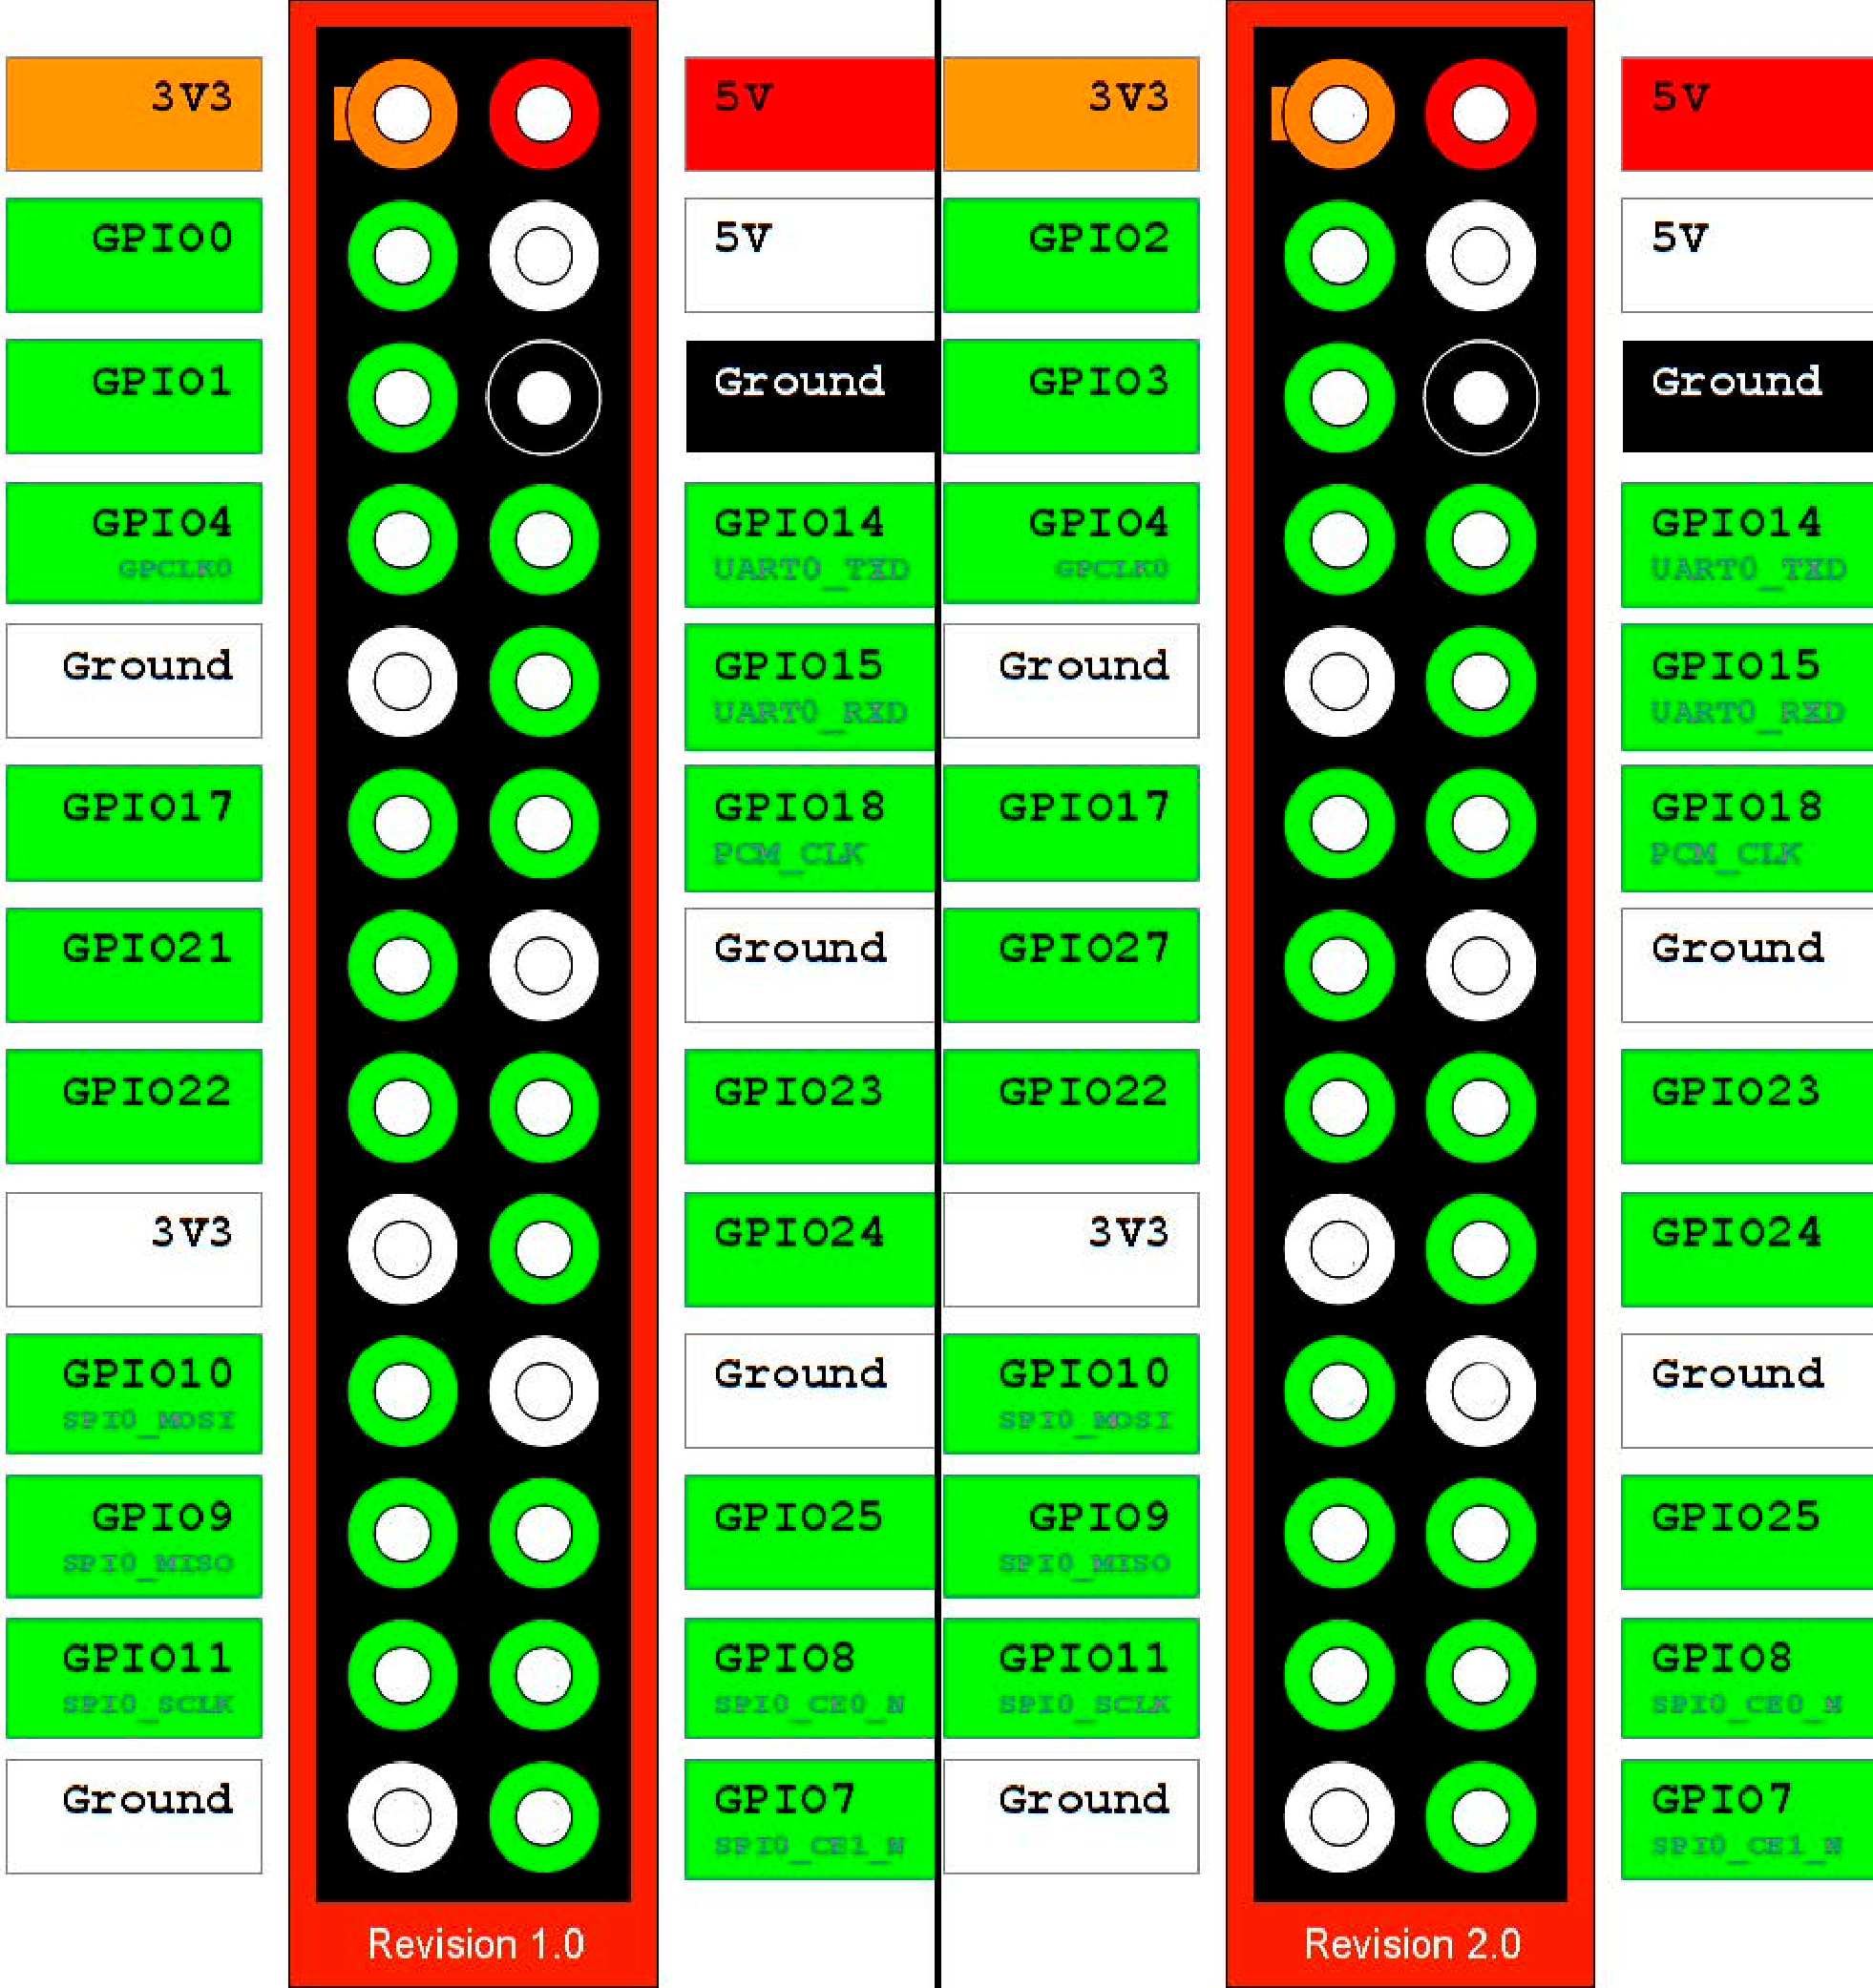
\includegraphics[scale=0.30]{pictures/iosharp/mapping-raspberrypi}
  \caption{Raspberry Pi pin mapping according to the GPIO\label{fig:mapping-rpi}}
\end{center}\end{figure}

The mapping has been divided into two classes, the first one maps the Pins so it will contain the naming according to the platform pins, in case of this thesis, both versions are mapped.
\\
The second file is used to pass the specific pins to the program, for example it configures the pins for the SPI or the UART. It is interesting to mention that in Linux the SPI and UART are known as devices so they are located under \verb!/dev/! directory. Raspberry Pi SPI device can have two slaves by using the \verb!spidev0.0! and \verb!spidev0.1!. This indicates that there are one device capable of having two slaves. The MISO, MOSI and SCLK pins are shared whereas each slave has its own chip select. In case of the UART it is also represented as a device and is named \verb!/dev/ttyAMA0! on the Raspberry Pi.
\chapter{Tests of IOSharp}\label{C:IOSharp Implementation}
Simultaneously with the development of IOSharp some small tests were created so the developed module could be tested to verify the properly operation. There are three major tests without taking into account the simple GPIO. First of all the SPI with the Interrupt port was tested using a RFID reader, secondly an Arduino and a RaspberryPi running IOSharp where connected via a Serial Port so one could send a message and the other forward to the first again. Finally HomeSense will be deployed on the RaspberryPi using IOSharp, and it will be compared with the original version of it, using the Netudino Mini.

\section{RFID and IOSharp}\label{S:rfid-iosharp}
This was the first test to verify the SPI and the Interruptions in a real environment using a RFID card reader connected through the SPI bus. In this case the code used for a Netduino has been taken and with minimal changes to the code it has been able to use without problems this reader.
\\
The card reader uses a MFRC522 chip from NXP and its hosted interfaces are SPI, UART and I$^{2}$C. In this case the chip is mounted on a PCB which offers the SPI connection, this reader is the MF522-AN from Mifare.

\subsection{Micro Framework and Netduino}\label{S:IOEx-SPI-Using-NETMF}
The original example uses a Netduino with the standard Micro Framework from Microsoft, then the RFID is connected through SPI to the board and a program will read the MFRC522 Version, then a timer will be configured to pull data from the card every 500 milliseconds. After pulling this data the program will try to identify the tag between the different Mifare versions and also print the serial number of the tag.


\subsection{Integrating IOSharp}\label{S:IOEx-SPI-Using-IOSharp}
 
\section{Arduino and IOSharp echoing}\label{S:rfid-iosharp}
\section{HomeSense over IOSharp}\label{S:HomeSense-IOSharp}
\section{Current IOSharp release}\label{S:current-iosharp-release}

%% Remove the final dot and print the glossaries
%\renewcommand*{\glspostdescription}{}
\printglossaries

%%%%%%%%%%%%%%%%%%%%%%%%%%%%%%%%%%%%%%%%%%%%%%%%%%%%%%%%%%%%%%%%%%%%%%%%%
%%%  BIBLIOGRAFIA
%%%%%%%%%%%%%%%%%%%%%%%%%%%%%%%%%%%%%%%%%%%%%%%%%%%%%%%%%%%%%%%%%%%%%%%%%%

%%% Per la bibliografia hi ha 2 opcions: generarla amb la utilitat BibTeX 
%%%                                      o fer-la ''a ma''
%%% NOTA: podeu trobar facilment informaci� sobre BibTeX a:
%%%  http://www.ctan.org/tex-archive/biblio/bibtex/contrib/doc/


%%% OPCIO 1: BibTeX -> descomentar les dues l�nies
%%% a)  Estil de bibliografia\\
%\bibliographystyle{unsrt}  
%%% b) Indicar els fitxers que contenen la bibliografia
%\bibliography{bibliography2}  

%%% OPCIO 2: bibliografia manual
%%%
%%% L'argument d'entrada es el numero de referencies que s'inclouen
\renewcommand{\bibname}{REFERENCES}
\begin{thebibliography}{9}

%% Llibres:  Autor/s (cognoms i inicials dels noms), t�tol del llibre (en cursiva), editor, ciutat i any de publicaci�. Quan es cita el cap�tol d'un llibre s'ha d'indicar el t�tol del cap�tol (entre cometes), el t�tol del llibre (en cursiva) i els n�meros de p�gines amb la primera i la darrera incloses.
%%  Exemple de capitol en llibre

\bibitem{cite:middleware}
Schmidt, D.C. and Schantz, R.E., "Middleware for Distributed System - Evolving the Common Structure for Network-centric Applications", {\it Encyclopedia of Software Eng.}, Wiley \& Sons, New York, 2001. Also available at \url{http://www.agentgroup.unimore.it/didattica/ingss/Lec_Middleware/Schmidt_Middleware.pdf}

\bibitem{cite:mom}
Bagula, A.B., Denko, M.K. and Zennaro, M., "Middleware for Mobile and Pervasive Services", Chap. 7 in {\it Handbook of mobile systems applications and services}, Taylor and Francis Group, Kumar, A. and Xie, B., pp. 248-249, Boca Raton (FL), 2012. 

\bibitem{cite:oom}
Khan, S., Qureshi, K. and Rashid, H., "Performance Comparison of ICE, HORB, CORBA and Dot 
NET Remoting Middleware Technologies", {\it International Journal of Computer Applications}, 3(11), 15-18 (2010). Also available at \url{http://www.ijcaonline.org/volume3/number11/pxc3871105.pdf}

\bibitem{cite:marea}
L�pez, J., Royo, P., Barrado, C., Pastor, E., "Applying marea middleware to UAS communications", {\it  In Proceedings of the AIAA Infotech@Aerospace Conference and AIAA Unmanned Unlimited Conference 2009}, Seattle (WH). Also available at \url{http://upcommons.upc.edu/e-prints/bitstream/2117/9248/1/infotech09.pdf}

\bibitem{cite:thesis-soa-avionics}
L�pez, J., "Service Oriented Architecture for Embedded (Avionics) Applications", {\it  The PhD Program on Computer Architecture Technical School of Castelldefels Technical University of Catalonia}, Barcelona, 2011. Also available at \url{https://dl.dropbox.com/u/2857619/thesis-small.pdf}

\bibitem{cite:delegate}  
Kiely, D., "Delegates Tutorial" in {\it The Microsoft Developer Network (MSDN)}. Available at \url{http://msdn.microsoft.com/en-us/library/aa288459(v=vs.71).aspx}

\bibitem{cite:serialization} 
Albahari, J. and Albahari B., "Serialization", Chap. 17 in {\it C\# 5.0 in a Nutshell: The definitive reference},
O`REILLY, Roumeliotis, R., pp. 691-728, Sebastopol (CA), 2012.

\bibitem{cite:performance-sockets} 
Kiely, D., "Get Closer to the Wire with High-Performance Sockets in .NET" in {\it The Microsoft Developer Network (MSDN) Magazine}. Available at \url{http://msdn.microsoft.com/es-es/magazine/cc300760(en-us).aspx}

\bibitem{cite:backporting}
Books Llc, Source Wikipedia, "Software Quality: Software Crisis, Kludge, Second-System Effect, Workaround, Reliability Engineering, Fault-Tolerant System", Books Llc, Memphis (Tennessee), 2011.

\end{thebibliography}

%%%%%%%%%%%%%%%%%%%%%%%%%%%%%%%%%%%%%%%%%%%%%%%%%%%%%%%%%%%%%%%%%%%%%%%%%%
%%%%%%                           APENDIXS                         %%%%%%%%
%%%%%%%%%%%%%%%%%%%%%%%%%%%%%%%%%%%%%%%%%%%%%%%%%%%%%%%%%%%%%%%%%%%%%%%%%%

\pagestyle{empty}  % no tocar

%% Descomentar una de les dues l�nies seg�ents, en funci� de:
%%  a) els apendixs s'encuadernaran apart (amb portada) 
%%  b) els apendixs s'enquadernen amb el mateix projecte (sense portada). 
%% Recordeu que si tot el document (amb ap�ndixs) excedeix les 100 pagines 
%% s'ha d'enquadernar a part
\appendix\ambportada
%\appendix\senseportada


%%%%%%%%%%%%%%%%%%%%%%%%%%%%%%%%%%%%%%%%%%%%%%%%%%%%%%%%%%%%%%%%%%%%%%%%%%
%%%%%% INCLOURE A PARTIR D'AQUI TOTS ELS CAP�TOLS DELS APENDIXS   %%%%%%%%
%%%%%%%%%%%%%%%%%%%%%%%%%%%%%%%%%%%%%%%%%%%%%%%%%%%%%%%%%%%%%%%%%%%%%%%%%%
\chapter{Technical information. Libraries and Datasheets}\label{C:Libraries-Datasheets}
\section{Library Types}\label{S:appendices-libraries-types}
Below are explained the different types of libraries, its characteristics and the different pros and cons of them.
\begin{itemize}
  \item 
  \textbf{Static Library}
  \\
  This kind of library is that one that is imported while programming, and when the source code is the library is linked statically in the generated binary, this means that the compiler takes the library functions used along the program and then are embedded statically to the compiled binary, in this way, the functions are fiscally located with the program. 
\\
For example, imagine that you create a library with 3 functions, called \verb!get_password()!, \verb!generate_token()! and \verb!hash(char[] plain())!,  but in the current project you only use two of this functions, which are \verb!get_password()! and \verb!get_token()!. When the compiler builds the project code will only take the functions from the library that are currently used in the program and then insert them into the binary. At this point, deleting that library won't affect the generated binary, and it will be able to use it without any dependency problems related to missing libraries (dependencies).
\\
The typical files for this type is .lib for Windows and .a for UNIX systems.
  
  \item
  \textbf{Dynamic Library}
  \\
  In order to avoid the replication of libraries that occurs in static ones, the dynamic libraries were created. This type of libraries is normally used along the operating systems to let applications use the offered functions and APIs written from the OS. In this case, and instead of the functional way of static libraries, any function from the library will be embedded on the generated binary, in this case is important to check that the dependencies are well satisfied when the binary is used, because a missing dependency will break the execution.

In this case, the usual extension files are .dll for Windows and .so for UNIX. But .so files are also used in Windows, especially in web browsers, which use this types of library to load browser plugins such us Flash.

There are two subtypes of dynamic libraries which are explained below:
  \begin{itemize}
    \item 
    \textbf{Dynamically Linked}
  	\\
  	These libraries must be available at compiling/link phase, because the compiler will verify that the function exists and that it is used properly. The libraries will be loaded at start time of the program. In this case, all the functions are mapped into the code.
    \item
    \textbf{Dynamically Loaded}
    \\
    Instead of the previous library, the dynamic loading is used by programs to load or unload libraries and use its functions at run time. When the program needs to use a function it loads the library, then it uses the required functions and finally the library is unloaded again.
    \end{itemize}
\end{itemize}

\textbf{Pros and cons}
\\
The main problem of using static libraries is that the compiled binary takes much more memory and the library is embedded in every program that needs some functions from that library. But, on the other hand, using static libraries the access to its functions by programs is much fast than dynamic ones. Using them also avoids dependency problems, because the dependencies are embedded instead of being located in the file system like dynamic ones.
\\
Regarding the dynamic libraries, they help to avoid replications and memory consumption, and also help to maintain the library updated in all programs that use them, although this can seem pretty good, it can have two bad effects into the generated program. First of all, if the library is missing in the system, the program will not run or will crash in execution time. Secondly, if the library is updated but some methods are changed, the program will crash because the non-existing function, and it will be necessary to readjust the code again, recompile and redistribute it.

\section{spidev.h}\label{S:linux-spi-spidev}
Source code of the library spidev.h used along this project. The different macros needed to configure the ioctl calls.
\begin{lstlisting}[language=C, caption={linux/spi/spidev.h}]
/*
 * include/linux/spi/spidev.h
 *
 * Copyright (C) 2006 SWAPP
 *      Andrea Paterniani <a.paterniani@swapp-eng.it>
 *
 * This program is free software; you can redistribute it and/or modify
 * it under the terms of the GNU General Public License as published by
 * the Free Software Foundation; either version 2 of the License, or
 * (at your option) any later version.
 *
 * This program is distributed in the hope that it will be useful,
 * but WITHOUT ANY WARRANTY; without even the implied warranty of
 * MERCHANTABILITY or FITNESS FOR A PARTICULAR PURPOSE.  See the
 * GNU General Public License for more details.
 *
 * You should have received a copy of the GNU General Public License
 * along with this program; if not, write to the Free Software
 * Foundation, Inc., 675 Mass Ave, Cambridge, MA 02139, USA.
  */

#ifndef SPIDEV_H
#define SPIDEV_H

#include <linux/types.h>

/* User space versions of kernel symbols for SPI clocking modes,
 * matching <linux/spi/spi.h>
 */

#define SPI_CPHA                0x01
#define SPI_CPOL                0x02

#define SPI_MODE_0              (0|0)
#define SPI_MODE_1              (0|SPI_CPHA)
#define SPI_MODE_2              (SPI_CPOL|0)
#define SPI_MODE_3              (SPI_CPOL|SPI_CPHA)

#define SPI_CS_HIGH             0x04
#define SPI_LSB_FIRST           0x08
#define SPI_3WIRE               0x10
#define SPI_LOOP                0x20
#define SPI_NO_CS               0x40
#define SPI_READY               0x80

/*---------------------------------------------------------------------------*/

/* IOCTL commands */

#define SPI_IOC_MAGIC                   'k'

struct spi_ioc_transfer {
        __u64           tx_buf;
        __u64           rx_buf;

        __u32           len;
        __u32           speed_hz;

        __u16           delay_usecs;
        __u8            bits_per_word;
        __u8            cs_change;
        __u32           pad;

        /* If the contents of 'struct spi_ioc_transfer' ever change
         * incompatibly, then the ioctl number (currently 0) must change;
         * ioctls with constant size fields get a bit more in the way of
         * error checking than ones (like this) where that field varies.
         *
         * NOTE: struct layout is the same in 64bit and 32bit userspace.
         */
};

/* not all platforms use <asm-generic/ioctl.h> or _IOC_TYPECHECK() ... */
#define SPI_MSGSIZE(N) \
        ((((N)*(sizeof (struct spi_ioc_transfer))) < (1 << _IOC_SIZEBITS)) \
                ? ((N)*(sizeof (struct spi_ioc_transfer))) : 0)
#define SPI_IOC_MESSAGE(N) _IOW(SPI_IOC_MAGIC, 0, char[SPI_MSGSIZE(N)])


/* Read / Write of SPI mode (SPI_MODE_0..SPI_MODE_3) */
#define SPI_IOC_RD_MODE                 _IOR(SPI_IOC_MAGIC, 1, __u8)
#define SPI_IOC_WR_MODE                 _IOW(SPI_IOC_MAGIC, 1, __u8)

/* Read / Write SPI bit justification */
#define SPI_IOC_RD_LSB_FIRST            _IOR(SPI_IOC_MAGIC, 2, __u8)
#define SPI_IOC_WR_LSB_FIRST            _IOW(SPI_IOC_MAGIC, 2, __u8)

/* Read / Write SPI device word length (1..N) */
#define SPI_IOC_RD_BITS_PER_WORD        _IOR(SPI_IOC_MAGIC, 3, __u8)
#define SPI_IOC_WR_BITS_PER_WORD        _IOW(SPI_IOC_MAGIC, 3, __u8)

/* Read / Write SPI device default max speed hz */
#define SPI_IOC_RD_MAX_SPEED_HZ         _IOR(SPI_IOC_MAGIC, 4, __u32)
#define SPI_IOC_WR_MAX_SPEED_HZ         _IOW(SPI_IOC_MAGIC, 4, __u32)



#endif /* SPIDEV_H */
\end{lstlisting}

\section{SPI Test. RFID Reader}\label{S:linux-spi-spidev}
\subsection{MFRC522 Datasheet}\label{SS:Libs-MFRC522-Datasheet}
The datasheet of this card card reader can be find at the NXP website or in the following link \url{http://www.nxp.com/documents/data_sheet/MFRC522.pdf}.
\\
\subsection{RFID Reader program}\label{SS:Libs-RFID-Reader}
\begin{lstlisting}[language=CSharp, caption={SPIExample.cs - RFID Reading interval}]
using System;
using System.Runtime.CompilerServices;
using System.Threading;
using IOSharp.Utils;
using System.Net;

namespace IOSharp.Exmples
{
    public class SPIExample
    {
        private MFRC522.SPIApi mfrc522 = new MFRC522.SPIApi();
        private bool onUpdate = false;
        private bool activated = false;
        private Timer cardReader = null;

        public static void Main()
        {
            new SPIExample().Run();
        }

        private void Run()
        {
            mfrc522.ConfigureSPI();
            StringUtils.PrintConsole("MF522-AN Version: "+StringUtils.ToHexString(mfrc522.ReadReg_MFRC522(mfrc522.VersionReg)));
            ConfigureTimer(!activated);
            Thread.Sleep(-1);
        }

        private void ConfigureTimer(bool activate)
        {
            if (activate)
            {
                Utils.StringUtils.PrintConsole("****Card reader started****");
                onUpdate = false;
                mfrc522.MFRC522Init();
                cardReader = new Timer(StartMFRC522, this, 0, 500);
                activated = true;

            }
            else
            {
                Utils.StringUtils.PrintConsole("****Card reader stoped****");
                cardReader.Dispose();
                mfrc522.MFRC522Stop();
                activated = false;
            }
        }

        private void StartMFRC522(Object timerInput)
        {
            if (!onUpdate)
            {
                onUpdate = true;
                String cardType = mfrc522.ReadTagTypeString(mfrc522.PICC_REQALL);
                if (!cardType.Equals("*"))
                {
                    CardDetected(cardType, mfrc522.ReadSerialNumberString());
                }
                onUpdate = false;
            }
        }

        private void CardDetected(String cardType, String serialNumber)
        {
            /**Card type
            *			 	0x4400 = Mifare_UltraLight
            *				0x0400 = Mifare_One(S50)
            *				0x0200 = Mifare_One(S70)
            *				0x0800 = Mifare_Pro(X)
            *				0x4403 = Mifare_DESFire
            */

            cardType = cardType.Trim();
            switch (cardType)
            {
                case "44 00":
                    cardType = "Mifare_UltraLight (" + cardType + ") ";
                    break;
                case "04 00":
                    cardType = "Mifare_One(S50) (" + cardType + ") ";
                    break;
                case "02 00":
                    cardType = "Mifare_One(S70) (" + cardType + ") ";
                    break;
                case "08 00":
                    cardType = "Mifare_Pro(X) (" + cardType + ") ";
                    break;
                case "44 03":
                    cardType = "Mifare_DESFire (" + cardType + ") ";
                    break;
            }
            StringUtils.PrintConsole("Card detected: " + cardType + "- Serial: " + serialNumber);
        }
    }
}
\end{lstlisting}

\section{AlterNative System Library}\label{SS:Libs-AlterNative}
\begin{figure}[H]\begin{center}
 \centering
  \captionsetup{justification=centering}
  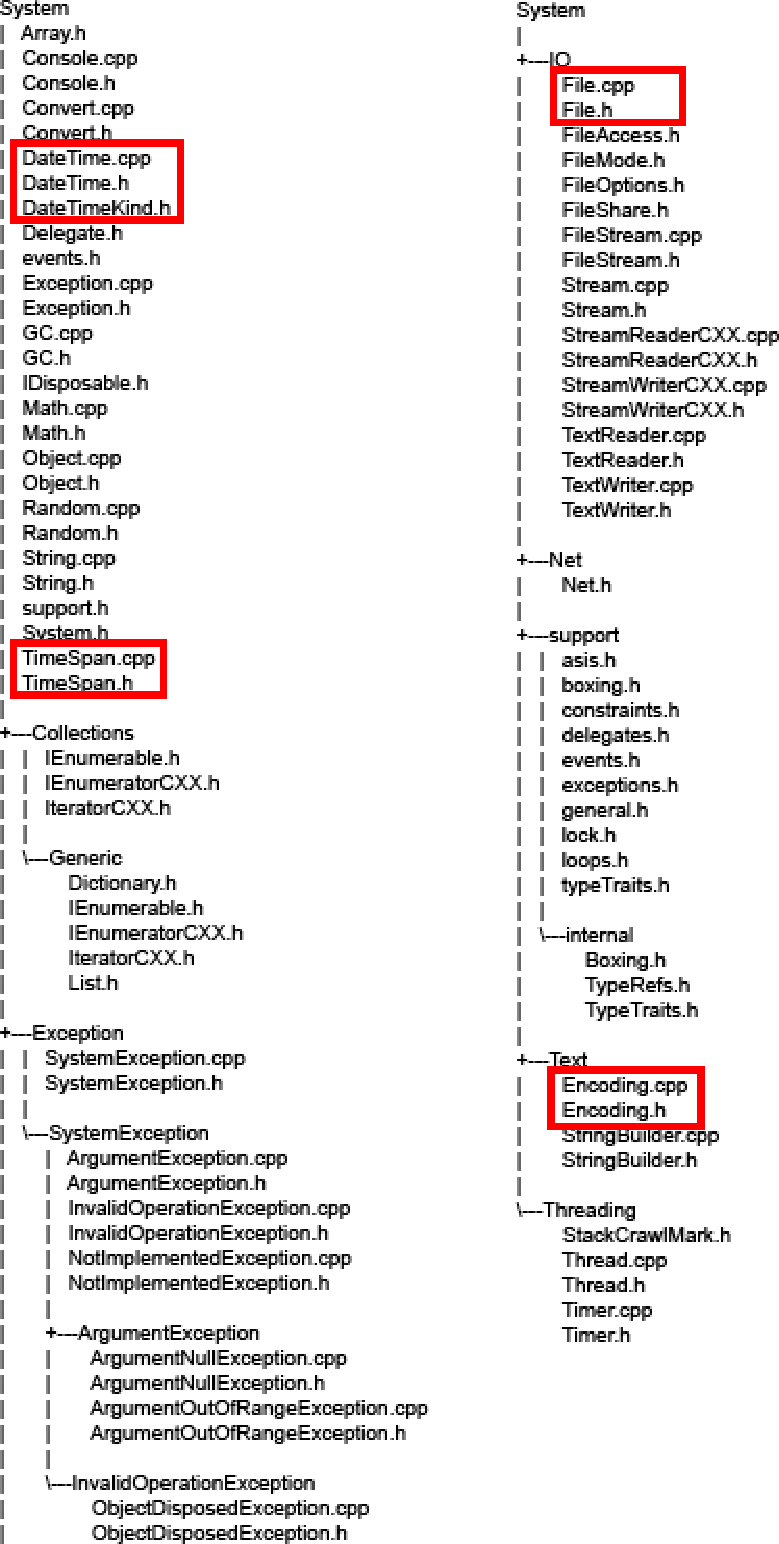
\includegraphics[width=0.75\textwidth]{pictures/appendices/alternative-cpp-classes}
  \caption{Tree dump of the C++ libraries of AlterNative currently implemented\label{fig:Libs-AlterNative}}
\end{center}\end{figure}


%%%%%%%%%%%%%%%%%%%%%%%%%%%%%%%%%%%%%%%%%%%%%%%%%%%%%%%%%%%%%%%%%%%%%%%%%%

%%%%%%%%%%%%%%%%%%%%%%%%%%%%%%%%%%%%%%%%%%%%%%%%%%%%%%%%%%%%%%%%%%%%%%%%%%
%%%%%%%%%%%%%%%%%%%%%%%%%%%%%%%%%%%%%%%%%%%%%%%%%%%%%%%%%%%%%%%%%%%%%%%%%%
%%%%%%%%%%%%%%%%%%%%%%%%%%%%%%%%%%%%%%%%%%%%%%%%%%%%%%%%%%%%%%%%%%%%%%%%%%
% i  aixo es tot! ;)
\cleardoublepage
\end{document}





